\chapter{Frobenius algebras}
\label{ch:frobenius}


\section{Three equivalent characterizations}
\label{sec:char-Frobenius}
We begin by recalling the essential algebraic notions, which will be necessary to give a proper definition of a Frobenius algebra. 
Through the chapter, we let $\Bbbk$ denote a field.

\begin{tcbdfn}[Algebras over a field]
    A \emph{$\Bbbk$-algebra} (i.e. an algebra over a field $\Bbbk$) is a $\Bbbk$-vector space $A$ equipped with two $\Bbbk$-linear maps 
    \[ \mu \colon A \tensor A \to \tensor A \qquad \eta \colon \Bbbk \to A  \]
    such that the following diagrams commute.
\[
\begin{tikzcd}
    & A \tensor A \tensor A \arrow[dl, "\mu \tensor \id_A", swap] \arrow[dr, "\id_A \tensor \mu"] & \\
    A \tensor A \arrow[dr, "\mu", swap] & & A \tensor A \arrow[dl, "\mu"] \\
    & A &
\end{tikzcd}
\]
% \[
% \begin{tikzcd}[column sep=5em]
% & A \tensor A \arrow[d, "\mu"] & \\
% \Bbbk \tensor A \arrow[ru, "\eta \tensor \id_A"] \arrow[r, "\sim", swap]&  A & A \tensor \Bbbk \arrow[lu, "\id_A \tensor \eta", swap] \arrow[l,"\sim"]  
% \end{tikzcd}
% \]
\[
\begin{tikzcd}
    & A \tensor A \arrow[rd, "\mu"] & & A \tensor A \arrow[ld, "\mu", swap]& \\
    \Bbbk \tensor A \arrow[ru, "\eta \tensor \id_A"] \arrow[rr, "\sim", swap]& & A & & A \tensor \Bbbk \arrow[lu, "\id_A \tensor \eta", swap] \arrow[ll,"\sim"]  
\end{tikzcd}
\]
We call $\mu$ the \emph{multiplication} and $\eta$ the \emph{unit map}.
\end{tcbdfn}

This definition is equivalent to the standard notion of a (unital associative) $\Bbbk$-algebra from linear algebra: a $\Bbbk$-vector space equipped with an associative and unital bilinear product. 
Concretely, we can see that:
\begin{enumerate}
    \item \emph{Distributivity} follows from requiring $\mu$ to be $\Bbbk$-linear.
    \item \emph{Associativity} and \emph{compatibility with scalar product} follow from the two commutative diagrams.
    \item The \emph{unit element} is defined by the image of $1 \in \Bbbk$ through $\eta$.
\end{enumerate}


\begin{remark}
    It is no coincidence that these diagrams seem similar to the ones appearing at the beginning of our thesis in \ref{dfn:monoidal_category}. 
    $\Bbbk$-algebras are indeed internal monoids in the monoidal category $(\mathbf{Vect}_\Bbbk, \tensor, \Bbbk)$, while (strict) monoidal categories are monoids in $(\mathbf{Cat}, \times, \mathbf{1})$. 
    We'll define what this means in the next chapter. (See \ref{dfn:internal-monoid})
\end{remark}

\begin{tcbdfn}[Homomorphisms of $\Bbbk$-algebras]
    Let $(A, \mu, \eta)$, $(A', \mu',\eta')$ be $\Bbbk$-algebras. A \emph{$\Bbbk$-algebra homomorphism} $\varphi \colon A \to A'$ is a $\Bbbk$-linear map that preserves the multiplication and unit structures. Concretely, the following diagrams are required to commute.
    \[
    \begin{tikzcd}
        A \tensor A \arrow[d, "\mu"] \arrow[r, "\varphi \tensor \varphi"] & A' \tensor A' \arrow[d, "\mu'"] \\
        A \arrow[r, "\varphi"] & A'
    \end{tikzcd}
    \qquad
    \begin{tikzcd}
        A \arrow[rr, "\varphi"] & & A' \\
        & \Bbbk \arrow[ul, "\eta"] \arrow[ur, "\eta'", swap] &
    \end{tikzcd}
    \]
\end{tcbdfn}

We can then denote with $\mathbf{Alg}_\Bbbk$ the category of $\Bbbk$-algebras and $\Bbbk$-algebra homomorphisms.

%%% eventuali def relative a spazi vettoriali

% \begin{tcbdfn}[Linear forms]
%     Let $V$ be any $\Bbbk$-vector space. A $\Bbbk$-linear map $V \to \Bbbk$ is called a \emph{linear form}. 
% \end{tcbdfn}

% \begin{tcbdfn}[Duals]
%     Let $V$ be any $\Bbbk$-vector space. 
% \end{tcbdfn}

% \begin{tcbdfn}[Pairings]
% \end{tcbdfn}

% \begin{tcbdfn}[Copairings]
%\end{tcbdfn}

% \begin{tcbdfn}[Non degenerate pairings]
% \end{tcbdfn}

% \begin{tcblemma}
% \end{tcblemma}


%%% eventuali def relative a moduli

% \begin{tcbdfn}[Right (left) A-modules]
% \end{tcbdfn}

We are now ready to state our first definition of a Frobenius algebras.

\begin{tcbdfn} \label{dfn:frobenius-algebra-a}
    A \emph{Frobenius algebra} is a finite dimensional $\Bbbk$-algebra $A$ equipped with a linear form $\varepsilon \colon A \to \Bbbk$, called the \emph{Frobenius form}, whose kernel $\{ x \in A \mid \varepsilon(a) = 0\}$ contains no nontrivial left ideals (i.e. only contains trivial ideals).
\end{tcbdfn}

Being a Frobenius algebra is a structure, not a property. That is, a given algebra can admit multiple Frobenius structures which must be specified. With an abuse of notation we will sometimes say $A$ is a Frobenius algebra; what we mean is we are assuming a Frobenius structure has been (or can be) chosen on A.

\begin{remark}
    The condition that $\ker(\varepsilon)$ has no nontrivial left ideal is equivalent to it not containing nontrivial \emph{principal} left ideals. 
    This is equivalent to saying that $\varepsilon(Ax) = 0$ implies $x=0$ for every $x \in A$.

    Moreover, this condition can be expressed equivalentely for right (principal) ideals.
\end{remark}

We now remember that any linear form $\Lambda \colon A \to \Bbbk$ canonically defines a bilinear pairing $p \colon A \tensor A \to \Bbbk$ by composing with the multiplication on $A$. More precisely we can send each $x \tensor y \in A \tensor A$ into $(\Lambda \circ \mu) (x \tensor y) = \Lambda(xy)$. By associativity of $\mu$, the pairing is itself associative, meaning $p(xy \tensor z) = p(x \tensor yz)$ for all $x, y, z \in A$. 

On the other hand, given an associative pairing $p \colon A \tensor A \to \Bbbk$ we can always canonically define a linear form $\Lambda \colon A \to \Bbbk$ by fixing $1_A$ as one of the entries. More precisely, we set $\Lambda(a) = p(1_A \tensor a) = p(a \tensor 1_A)$.

One can easily check these constructions are inverse to each other, giving a one-to-one correspondence between the two. A less obvious result is the following.

\begin{tcblemma}
Let A be a finite dimensional $\Bbbk$-algebra. An associative pairing $A \tensor A \to \Bbbk$ is non-degenerate if and only if the corresponding linear form $A \to \Bbbk$ is a Frobenius form.
\end{tcblemma}

This directly leads to an equivalent characterization of a Frobenius algebra.

\begin{tcbdfn}\label{dfn:frobenius-algebra-b}
    A \emph{Frobenius algebra} is a finite dimensional $\Bbbk$-algebra $A$ equipped with a non-degenerate associative pairing $\beta \colon A \tensor A \to \Bbbk$, called the \emph{Frobenius pairing}.
\end{tcbdfn}


% \begin{remark}
% Asking for a non-degenerate pairing $\beta \colon A \tensor A \to \Bbbk$ implies the existence of a \emph{copairing} $\gamma \colon \Bbbk \to A \tensor A$. We could then state the definition through such dual notion.
% \end{remark}
\todo[inline]{copairing??}


A non-degenerate pairing $\beta \colon A \tensor A \to \Bbbk$ induces canonical $\Bbbk$-linear isomorphisms $A \xrightarrow{\sim} A^*$ and $A^* \xrightarrow{\sim} A$. The associativity of $\beta$ is equivalent to the A-linearity of these isomorphisms (with respect to the appropriate left or right module structure). The two equivalent characterizations following from such properties won't be of use for our thesis, nonetheless we include them for completeness.

\begin{tcbdfn}\label{dfn:Frobenius-useless}
    A \emph{Frobenius algebra} is a finite dimensional $\Bbbk$-algebra $A$ equipped with a left $A$-linear isomorphism to its dual.
\end{tcbdfn}

\begin{tcbdfn}
    A \emph{Frobenius algebra} is a finite dimensional $\Bbbk$-algebra $A$ equipped with a right $A$-linear isomorphism to its dual.
\end{tcbdfn}


\todo[inline]{in realtà si potrebbe verificare che avere il pairing implica la dimensione finita... vale la pena dirlo? se sì come?}

Our discussion has so far focused on algebras. We now introduce their dual concept by reversing all the arrows.

\begin{tcbdfn}[Coalgebras over a field]
A $\Bbbk$-coalgebra (i.e. a coalgebra over a field $\Bbbk$) is a $\Bbbk$-vector space $A$ equipped with two $\Bbbk$-linear maps
\[
\delta \colon A \to A \tensor A \qquad \varepsilon \colon A \to \Bbbk
\]
such that the following diagrams commute
\[
\begin{tikzcd}
    & A \tensor A \tensor A & \\
    A \tensor A \arrow[ur, "\delta \tensor \id_A"] & & A \tensor A \arrow[ul, "\id_A \tensor \delta", swap] \\
    & A \arrow[ul, "\delta"] \arrow[ur, "\delta", swap] &
\end{tikzcd}
\]
\[
\begin{tikzcd}
    & A \tensor A \arrow[dl, "\varepsilon \tensor \id_A", swap] & & A \tensor A \arrow[dr, "\id_A \tensor \varepsilon"] & \\
    \Bbbk \tensor A & & A \arrow[ul, "\delta", swap] \arrow[ur, "\delta"] \arrow[ll, "\sim", swap] \arrow[rr, "\sim"] & & A \tensor \Bbbk
\end{tikzcd}
\]
We call $\delta$ the \emph{comultiplication} and $\varepsilon$ the \emph{counit map}.
\end{tcbdfn}

\begin{tcbdfn}
Let $(A, \delta, \varepsilon)$, $(A', \delta', \varepsilon')$ be $\Bbbk$-coalgebras. A \emph{$\Bbbk$-coalgebra homomorphism} $\phi \colon A \to A'$ is a $\Bbbk$-linear map that preserves the comultiplication and counit structures.
Concretely, the following diagrams are required to commute.
\[
\begin{tikzcd}
    A \tensor A \arrow[r, "\phi \tensor \phi"] & A' \tensor A' \\
    A \arrow[r, "\phi"] \arrow[u, "\delta", swap] & A' \arrow[u, "\delta'", swap]
\end{tikzcd}
\qquad
\begin{tikzcd}
    A \arrow[rr, "\phi"] \arrow[dr, "\varepsilon", swap] & & A' \arrow[dl, "\varepsilon'"]\\
    & \Bbbk &
\end{tikzcd}
\]
\end{tcbdfn}

We can hence state the last equivalent characterization.

\begin{tcbdfn}\label{dfn:frobenius-algebra-c}
A \emph{Frobenius algebra} is a $\Bbbk$-vector space $A$ equipped with both an algebra $(A, \mu, \eta)$ and a coalgebra $(A, \delta, \varepsilon)$ structure, such that the Frobenius relation, which corresponds to the commutativity of the diagrams below, holds.
\[
\begin{tikzcd}
    A \tensor A \arrow[d,"\mu"] \arrow[r, "\delta \tensor \id_A"] & A \tensor A \tensor A \arrow[d, "\id_A \tensor \mu"] \\
    A \arrow[r,"\delta"] & A \tensor A
\end{tikzcd}
\qquad
\begin{tikzcd}
    A \tensor A \arrow[d,"\mu"] \arrow[r, "\id_A \tensor \delta"] & A \tensor A \tensor A \arrow[d, "\mu \tensor \id_A"] \\
    A \arrow[r,"\delta"] & A \tensor A
\end{tikzcd}
\]
\end{tcbdfn}

Proving this last definition is not immediate when using this notation. To help ourselves in handling this proof we will introduce \emph{graphical calculus} in section \ref{sec:doodles}.

Finally, we define what it means to ask a Frobenius algebra to be symmetric. To do so we recall the three characterizations (even if we've not proved their equivalence yet) we'll work with from now on and state the notion of symmetry for each of these frameworks.

\begin{tcbdfn}[Frobenius algebras]
    \label{dfn:Frobenius-algebra-all}
    A \emph{Frobenius algebra} is a (finite dimensional) $\Bbbk$-algebra $A$ equippped with either:
    \begin{enumerate}[label=(\roman*), parsep=0pt]
        \item A linear form $\varepsilon \colon A \to \Bbbk$ whose kernel contains no nontrivial (left) ideals. \par [See definition \ref{dfn:frobenius-algebra-a}]
        \item A non-degenerate associative pairing $\beta \colon A \tensor A \to \Bbbk$ (and a copairing $\gamma \colon \Bbbk\to A \tensor A$). \par [See definition \ref{dfn:frobenius-algebra-b}]
        \item A coalgebra structure $(A, \delta, \varepsilon)$ satisfying the Frobenius relation. \par [See definition \ref{dfn:frobenius-algebra-c}]
    \end{enumerate}
\end{tcbdfn}

\begin{tcbdfn}[Commutative Frobenius algebras]
    A Frobenius algebra $A$ is \emph{commutative} if its underlying algebra structure is commutative.
\end{tcbdfn}

\todo[inline]{is it worth to mention symmetric Frob. algebras?}

% For completeness we also define an important class of Frobenius algebras.

% \begin{tcbdfn}[Symmetric Frobenius algebras]
%     A Frobenius algebra $A$ is \emph{symmetric} if one of the following (equivalent) conditions holds:
%     \begin{enumerate}
%         \item The Frobenius form $\varepsilon \colon A \to \Bbbk$ is central, meaning that $\varepsilon(ab)=\varepsilon(ba)$ for every $a, b \in A$.
%         \item The pairing $\beta \colon A \tensor A \to \Bbbk$ is symmetric, meaning $\beta(a \tensor b) = \beta(b \tensor a)$ for every $a, b \in A$.
%         \item The counit $\varepsilon$ is central.
%     \end{enumerate}
% \end{tcbdfn}

% It seems superflous (and in fact it is) to list the third condition separately, as it coincides with the first. We include it to maintain a consistent reference to the three characterizations above. 

% We also remind that since being a Frobenius algebra is a structure, the property of symmetry relates to such structure. We could then have two Frobenius structure on an algebra $A$ and have only one of them to be symmetric.

% We shall not confuse the notions of symmetry and commutativity. A \emph{commutative Frobenius algebra} is indeed just a Frobenius algebra whose underlying algebra is commutative. We then have that all commutative Frobenius algebras are symmetric, while the viceversa does not hold.

% \begin{remark}
%     We previously mentioned a fourth characterization of Frobenius algebra [See Definition \ref{dfn:Frobenius-useless}]. The notion of symmetry can also be formulated in that context by asking for the left (resp. right) $A$-linear isomorphism to be also right (resp. left) $A$-linear.
% \end{remark}

\section{Rigorous doodles} 
\label{sec:doodles}

%% Alternative titolo: 
% "Drawing conclusions"?? (ma non sto concludendo nulla)
% "Reading between the lines"

The aim of this section is to define a graphical language that will help us see more clearly the equivalence between the various definitions of Frobenius algebras.  \todo[inline]{add a note about such choice. kock used bordisms, why do we like wires?}

Through this section, we'll adopt these drawings as formal notations corresponding to $\Bbbk$-linear maps $A^m \to A^n$. The tensor product of two maps will correspond to placing the diagrams \emph{in parallel} (one above the other), while the composition will be represented by connecting them \emph{in series} (by simply connecting the wires).

\subsection{From pairing to Frobenius relation}
We hence begin by drawing the maps defining a $\Bbbk$-algebra as \emph{wires}.
\[
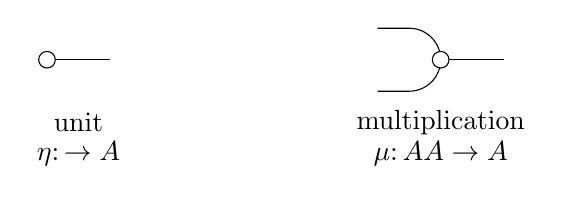
\begin{tikzpicture}
    \begin{scope}[x=0.8cm, y=0.4cm]
        \draw (0,0) -- (1,0);
        \draw[fill=white] (0,0) circle (3pt);
        \node (t1) at (0.5,-2) {unit};
        \node (t2) at (0.5,-3) {$\eta \colon \Bbbk \to A$};
    \end{scope}
    \begin{scope}[xshift=5cm,x=0.8cm, y=0.4cm]
    \draw[rounded corners=0.4cm] (-1,1) -- (0,1) -- (0,0);
    \draw[rounded corners=0.4cm] (-1,-1) -- (0,-1) -- (0,0);
    \draw (0,0) -- (1,0);
    \draw[fill=white] (0,0) circle (3pt);   
    \node (t1) at (0,-2) {multiplication};
    \node (t2) at (0,-3) {$\mu \colon A \tensor A \to A$};
    \end{scope}
\end{tikzpicture}
\]

We are now able to express the axioms of a $\Bbbk$-algebra graphically.

\[
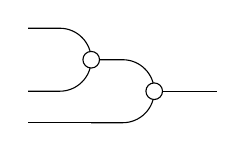
\begin{tikzpicture}[x=0.8cm, y=0.4cm, baseline]
    \draw[rounded corners=0.4cm] (-2,2) -- (-1,2) -- (-1,1);
    \draw[rounded corners=0.4cm] (-2,0) -- (-1,0) -- (-1,1);
    \draw[rounded corners=0.4cm] (-1,1) -- (0,1) -- (0,0);
    \draw[rounded corners=0.4cm] (-1,-1) -- (0,-1) -- (0,0);
    \draw (0,0) -- (1,0);
%    \draw plot [smooth, tension=2] coordinates {(0,0) (-.5,-1) (-1,-1.5) (-2,-2)};
%    \draw (-2,-2) to [bend right] (-1,-1);
    \draw (-1,-1) -- (-2,-1);
    \draw[fill=white] (-1,1) circle (3pt);   
    \draw[fill=white] (0,0) circle (3pt);  
\end{tikzpicture}
\quad=\quad
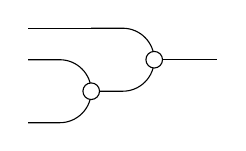
\begin{tikzpicture}[x=0.8cm, y=0.4cm, baseline]
    \draw[rounded corners=0.4cm] (-2,-2) -- (-1,-2) -- (-1,-1);
    \draw[rounded corners=0.4cm] (-2,0) -- (-1,0) -- (-1,-1);
    \draw[rounded corners=0.4cm] (-1,1) -- (0,1) -- (0,0);
    \draw[rounded corners=0.4cm] (-1,-1) -- (0,-1) -- (0,0);
    \draw (0,0) -- (1,0);
    \draw (-1,1) -- (-2,1);
    \draw[fill=white] (-1,-1) circle (3pt);   
    \draw[fill=white] (0,0) circle (3pt);   
\end{tikzpicture}
\hspace{3em}
\text{(associativity of $\mu$)}
\]

\[
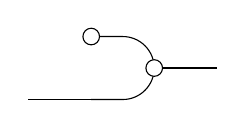
\begin{tikzpicture}[x=0.8cm, y=0.4cm, baseline]
    \draw[rounded corners=0.4cm] (-1,1) -- (0,1) -- (0,0);
    \draw[rounded corners=0.4cm] (-1,-1) -- (0,-1) -- (0,0);
    \draw (-1,-1) -- (-2,-1);
    \draw (0,0) -- (1,0);
    \draw[fill=white] (0,0) circle (3pt);
    \draw[fill=white] (-1,1) circle (3pt);
\end{tikzpicture}
\quad=\quad
\begin{tikzpicture}[x=0.8cm, y=0.4cm, baseline]
    \draw (0,0) -- (1,0);    
\end{tikzpicture}
\quad=\quad
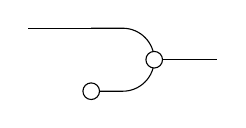
\begin{tikzpicture}[x=0.8cm, y=0.4cm, baseline]
    \draw[rounded corners=0.4cm] (-1,1) -- (0,1) -- (0,0);
    \draw[rounded corners=0.4cm] (-1,-1) -- (0,-1) -- (0,0);
    \draw (-1,1) -- (-2,1);
    \draw (0,0) -- (1,0);
    \draw[fill=white] (0,0) circle (3pt);
    \draw[fill=white] (-1,-1) circle (3pt);
\end{tikzpicture}
\hspace{3em}
\text{(unit axiom)}
\]

To then define a Frobenius algebra, through the first characterizazion, we need to define a Frobenius form $\varepsilon \colon A \to \Bbbk$, which will induce a Frobenius pairing $\beta \colon A \tensor A \to \Bbbk$.

\[
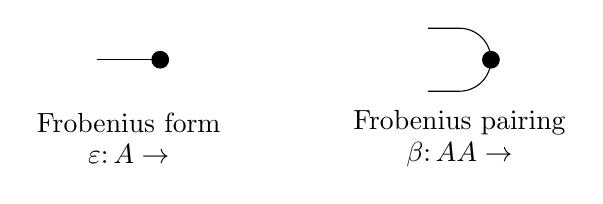
\begin{tikzpicture}
    \begin{scope}[x=0.8cm, y=0.4cm]
        \draw (0,0) -- (1,0);
        \draw[fill=black] (1,0) circle (3pt);
        \node (t1) at (0.5,-2) {Frobenius form};
        \node (t2) at (0.5,-3) {$\varepsilon \colon A \to \Bbbk$};
    \end{scope}
    \begin{scope}[xshift=5cm,x=0.8cm, y=0.4cm]
    \draw[rounded corners=0.4cm] (-1,1) -- (0,1) -- (0,0);
    \draw[rounded corners=0.4cm] (-1,-1) -- (0,-1) -- (0,0);
    \draw[fill=black] (0,0) circle (3pt);   
    \node (t1) at (-.5,-2) {Frobenius pairing};
    \node (t2) at (-.5,-3) {$\beta \colon A \tensor A \to \Bbbk$};
    \end{scope}
\end{tikzpicture}
\]

This relation can be explaned graphically as follows.

\[
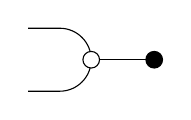
\begin{tikzpicture}[x=0.8cm, y=0.4cm, baseline]
    \draw[rounded corners=0.4cm] (-1,1) -- (0,1) -- (0,0);
    \draw[rounded corners=0.4cm] (-1,-1) -- (0,-1) -- (0,0);
    \draw (0,0) -- (1,0);
    \draw[fill=white] (0,0) circle (3pt); 
    \draw[fill=black] (1,0) circle (3pt); 
\end{tikzpicture}
\quad=\colon\quad
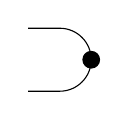
\begin{tikzpicture}[x=0.8cm, y=0.4cm, baseline]
    \draw[rounded corners=0.4cm] (-1,1) -- (0,1) -- (0,0);
    \draw[rounded corners=0.4cm] (-1,-1) -- (0,-1) -- (0,0);
    \draw[fill=black] (0,0) circle (3pt);   
\end{tikzpicture}
\hspace{3em}
\text{(defining $\beta$ from $\varepsilon$)}
\]
\[
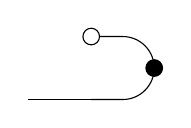
\begin{tikzpicture}[x=0.8cm, y=0.4cm, baseline]
    \draw[rounded corners=0.4cm] (-1,1) -- (0,1) -- (0,0);
    \draw[rounded corners=0.4cm] (-1,-1) -- (0,-1) -- (0,0);
    \draw (-1,-1) -- (-2,-1);
    \draw[fill=black] (0,0) circle (3pt);
    \draw[fill=white] (-1,1) circle (3pt);
\end{tikzpicture}
\quad=\colon\quad
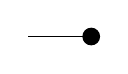
\begin{tikzpicture}[x=0.8cm, y=0.4cm, baseline]
    \draw (0,0) -- (1,0); 
    \draw[fill=black] (1,0) circle (3pt);   
\end{tikzpicture}
\quad\colon=\quad
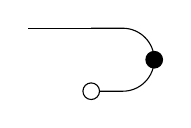
\begin{tikzpicture}[x=0.8cm, y=0.4cm, baseline]
    \draw[rounded corners=0.4cm] (-1,1) -- (0,1) -- (0,0);
    \draw[rounded corners=0.4cm] (-1,-1) -- (0,-1) -- (0,0);
    \draw (-1,1) -- (-2,1);
    \draw[fill=black] (0,0) circle (3pt);
    \draw[fill=white] (-1,-1) circle (3pt);
\end{tikzpicture}
\hspace{3em}
\text{(defining $\varepsilon$ from $\beta$)}
\]

Combining the associativity of the multiplication and the first of the above relations we obtain the associativity for the pairing.

\[
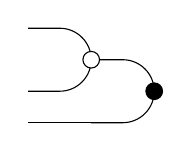
\begin{tikzpicture}[x=0.8cm, y=0.4cm, baseline]
    \draw[rounded corners=0.4cm] (-2,2) -- (-1,2) -- (-1,1);
    \draw[rounded corners=0.4cm] (-2,0) -- (-1,0) -- (-1,1);
    \draw[rounded corners=0.4cm] (-1,1) -- (0,1) -- (0,0);
    \draw[rounded corners=0.4cm] (-1,-1) -- (0,-1) -- (0,0);
%    \draw plot [smooth, tension=2] coordinates {(0,0) (-.5,-1) (-1,-1.5) (-2,-2)};
%    \draw (-2,-2) to [bend right] (-1,-1);
    \draw (-1,-1) -- (-2,-1);
    \draw[fill=white] (-1,1) circle (3pt);   
    \draw[fill=black] (0,0) circle (3pt);  
\end{tikzpicture}
\quad=\quad
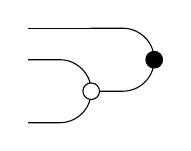
\begin{tikzpicture}[x=0.8cm, y=0.4cm, baseline]
    \draw[rounded corners=0.4cm] (-2,-2) -- (-1,-2) -- (-1,-1);
    \draw[rounded corners=0.4cm] (-2,0) -- (-1,0) -- (-1,-1);
    \draw[rounded corners=0.4cm] (-1,1) -- (0,1) -- (0,0);
    \draw[rounded corners=0.4cm] (-1,-1) -- (0,-1) -- (0,0);
    \draw (-1,1) -- (-2,1);
    \draw[fill=white] (-1,-1) circle (3pt);   
    \draw[fill=black] (0,0) circle (3pt);   
\end{tikzpicture}
\hspace{3em}
\text{(associativity of $\beta$)}
\]

Finally to obtain a Frobenius algebra we need the pairing to be non-degenerate. This means asking  for the existence of a \emph{copairing} $\gamma \colon \Bbbk \to A \tensor A$ such that the compositions $(\id_A \tensor \beta) \circ (\gamma \tensor \id_A)$ and $(\beta \tensor \id_A) \circ (\id_A \tensor \gamma)$ equal the identity. We can translate such requirements in graphical terms.
\[
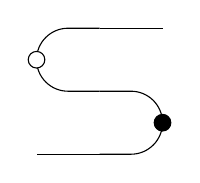
\begin{tikzpicture}[x=0.8cm, y=0.4cm, baseline]
    \draw[rounded corners=0.4cm] (0,0)--(-1,0)--(-1,1);
    \draw[rounded corners=0.4cm] (0,2)--(-1,2)--(-1,1);
    \draw[rounded corners=0.4cm] (1,-1)--(1,0)--(0,0);
    \draw[rounded corners=0.4cm] (1,-1)--(1,-2)--(0,-2);
    \draw (0,2)--(1,2);
    \draw (0,-2)--(-1,-2);
    \draw[fill=white] (-1,1) circle (3pt);   
    \draw[fill=black] (1,-1) circle (3pt);   
\end{tikzpicture}
\quad=\quad
\begin{tikzpicture}[x=0.8cm, y=0.4cm, baseline]
    \draw (0,0) -- (1,0);    
\end{tikzpicture}
\quad=\quad
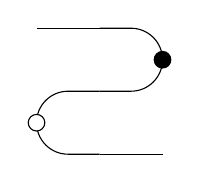
\begin{tikzpicture}[x=0.8cm, y=0.4cm, baseline]
    \draw[rounded corners=0.4cm] (0,0)--(1,0)--(1,1);
    \draw[rounded corners=0.4cm] (0,2)--(1,2)--(1,1);
    \draw[rounded corners=0.4cm] (-1,-1)--(-1,0)--(0,0);
    \draw[rounded corners=0.4cm] (-1,-1)--(-1,-2)--(-0,-2);
    \draw (0,2)--(-1,2);
    \draw (0,-2)--(1,-2);
    \draw[fill=white] (-1,-1) circle (3pt);   
    \draw[fill=black] (1,1) circle (3pt);   
\end{tikzpicture}
\hspace{3em}
\begin{tabular}{l}
      (non-degeneracy of $\beta$ \\ 
      or \emph{snake relation})
    \end{tabular}
\]

\begin{dfnx*}[Uniqueness of the copairing]
We can prove that the copairing $\gamma$ is unique, just through graphical calculus (we'll still include the commutative diagrams on the side, to emphasize how the two approaches corresponds). Suppose there exist two different copairings $\gamma$, $\xi$ satisfying such non-degeneracy condition.
We distinguish them graphically by drawing a white circle for $\gamma$ and a white square for $\xi$.
%$\copairing$, $\varcopairing$
We then have:
\[
% \begin{tikzpicture}[x=0.8cm, y=0.4cm, baseline]
%     \draw[rounded corners=0.4cm] (0,0)--(1,0)--(1,1);
%     \draw[rounded corners=0.4cm] (0,2)--(1,2)--(1,1);
%     \draw[rounded corners=0.4cm] (-1,-1)--(-1,0)--(0,0);
%     \draw[rounded corners=0.4cm] (-1,-1)--(-1,-2)--(-0,-2);
%     \draw (0,2)--(-1,2);
%     \draw (0,-2)--(1,-2);
%     \draw[fill=white] (-1,-1) circle (3pt);   
%     \draw[fill=black] (1,1) circle (3pt);   
% \end{tikzpicture}
% \quad = \quad
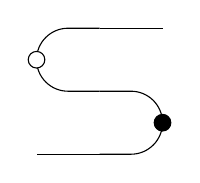
\begin{tikzpicture}[x=0.8cm, y=0.4cm, baseline]
    \draw[rounded corners=0.4cm] (0,0)--(-1,0)--(-1,1);
    \draw[rounded corners=0.4cm] (0,2)--(-1,2)--(-1,1);
    \draw[rounded corners=0.4cm] (1,-1)--(1,0)--(0,0);
    \draw[rounded corners=0.4cm] (1,-1)--(1,-2)--(0,-2);
    \draw (0,2)--(1,2);
    \draw (0,-2)--(-1,-2);
    \draw[fill=white] (-1,1) circle (3pt);   
    \draw[fill=black] (1,-1) circle (3pt);   
\end{tikzpicture}
\quad=\quad
\begin{tikzpicture}[x=0.8cm, y=0.4cm, baseline]
    \draw (0,0) -- (1,0);    
\end{tikzpicture}
\quad=\quad
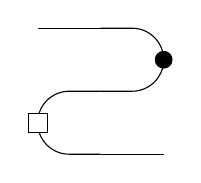
\begin{tikzpicture}[x=0.8cm, y=0.4cm, baseline]
    \draw[rounded corners=0.4cm] (0,0)--(1,0)--(1,1);
    \draw[rounded corners=0.4cm] (0,2)--(1,2)--(1,1);
    \draw[rounded corners=0.4cm] (-1,-1)--(-1,0)--(0,0);
    \draw[rounded corners=0.4cm] (-1,-1)--(-1,-2)--(-0,-2);
    \draw (0,2)--(-1,2);
    \draw (0,-2)--(1,-2);
    \draw[fill=white] (-1.15,-1.3) rectangle (-0.85,-0.7);   
    \draw[fill=black] (1,1) circle (3pt);   
\end{tikzpicture}
% \quad = \quad
% \begin{tikzpicture}[x=0.8cm, y=0.4cm, baseline]
%     \draw[rounded corners=0.4cm] (0,0)--(-1,0)--(-1,1);
%     \draw[rounded corners=0.4cm] (0,2)--(-1,2)--(-1,1);
%     \draw[rounded corners=0.4cm] (1,-1)--(1,0)--(0,0);
%     \draw[rounded corners=0.4cm] (1,-1)--(1,-2)--(0,-2);
%     \draw (0,2)--(1,2);
%     \draw (0,-2)--(-1,-2);
%     \draw[fill=white] (-1.15,0.7) rectangle (-.85,1.3);   
%     \draw[fill=black] (1,-1) circle (3pt);   
% \end{tikzpicture}
\hspace{3em}
\begin{tikzcd}
    & A \tensor A \tensor A \arrow[dr, "\id_A \tensor \beta"] & \\
    A \arrow[rr, "\id_A"] \arrow[ur, "\gamma \tensor \id_A"] \arrow[dr, "\id_A \tensor \xi", swap] & & A \\
    & A \tensor A \tensor A \arrow[ur, "\beta \tensor \id_A", swap] &
\end{tikzcd}
\]

By considering the tensor of the the two copairings and composing it with $\id_A \tensor \beta \tensor \id_A$, we obtain through the above relations, the following:

\[
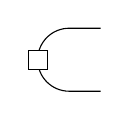
\begin{tikzpicture}[x=0.8cm, y=0.4cm, baseline]
    \draw[rounded corners=0.4cm] (0,0)--(0,1)--(1,1);
    \draw[rounded corners=0.4cm] (0,0)--(0,-1)--(1,-1);
    \draw[fill=white] (-0.15,-0.3) rectangle (.15,.3);   
\end{tikzpicture}
\quad = \quad
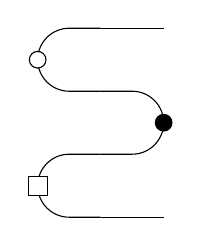
\begin{tikzpicture}[x=0.8cm, y=0.4cm, baseline]
    \draw[rounded corners=0.4cm] (0,0)--(0,1)--(-1,1);
    \draw[rounded corners=0.4cm] (0,0)--(0,-1)--(-1,-1);
    \draw[rounded corners=0.4cm] (-1,1)--(-2,1)--(-2,2);
    \draw[rounded corners=0.4cm] (-2,2)--(-2,3)--(-1,3);
    \draw[rounded corners=0.4cm] (-1,-1)--(-2,-1)--(-2,-2);
    \draw[rounded corners=0.4cm] (-2,-2)--(-2,-3)--(-1,-3);
    \draw (-1,3)--(0,3);
    \draw (-1,-3)--(0,-3);
    \draw[fill=white] (-2.15,-2.3) rectangle (-1.85,-1.7);   
    \draw[fill=black] (0,0) circle (3pt);   
    \draw[fill=white] (-2,2) circle (3pt);
\end{tikzpicture}
\quad = \quad
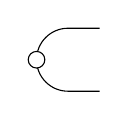
\begin{tikzpicture}[x=0.8cm, y=0.4cm, baseline]
    \draw[rounded corners=0.4cm] (0,0)--(0,1)--(1,1);
    \draw[rounded corners=0.4cm] (0,0)--(0,-1)--(1,-1);
    \draw[fill=white] (0,0) circle (3pt);
\end{tikzpicture}
\]
and the correspondig commutative diagram below.
\[
\begin{tikzcd}[column sep=5em, row sep=3em]
    & A \tensor A \arrow[d, "\textcolor{red}{\gamma \tensor \id_A} \tensor \id_A"] \arrow[dr, "\textcolor{red}{\id_A} \tensor \id_A", bend left=30] & \\
    \Bbbk \arrow[r, "\gamma \tensor \xi"] \arrow[ur, "\xi", bend left=30] \arrow[dr, "\gamma", swap, bend right=30] & A \tensor A \tensor A \tensor A \arrow[r, "\textcolor{red}{\id_A \tensor} \textcolor{violet}{\beta} \textcolor{blue}{\tensor \id_A}"] & A \tensor A \\
    & A \tensor A \arrow[u, "\id_A \tensor \textcolor{blue}{\id_A \tensor \xi}"] \arrow[ur, "\id_A \tensor \textcolor{blue}{\id_A}", swap, bend right=30] &
\end{tikzcd}
\]
We conclude $\gamma = \xi$, proving uniqueness.
We can see, just by this small example, how the graphical approach is way more straightforward, compared to the diagrammatic one, which easily becomes messy.
\end{dfnx*}


We are now ready to prove the definition of a Frobenius algebra through a non-degenerate associative pairing gives rise to a coalgebra satisfying the Frobenius relation. 
\todo[inline]{Maybe we can write this as a lemma}

\textbf{(Defining a comultiplication).} Since the multiplication is defined as $\wiremult$, we would want the comultiplication to be something like $\wirecomult$ satisfying the coalgebra axioms.

Before doing so, by recalling the associativity of the pairing $\beta$, we define $\phi = (\mu \tensor \id_A) \circ \beta = (\id_A \tensor \mu) \circ \beta$. 
Looking at its graphical representation, we'll call it the \emph{trident map}. 

\[
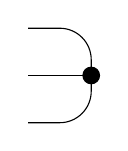
\begin{tikzpicture}[x=0.8cm, y=0.4cm, baseline]
    \draw[rounded corners=0.4cm] (0,0)--(0,1.5)--(-1,1.5);
    \draw[rounded corners=0.4cm] (0,0)--(0,-1.5)--(-1,-1.5);
    \draw (0,0)--(-1,0);
    \draw[fill=black] (0,0) circle (3pt);   
\end{tikzpicture}
\quad=\quad
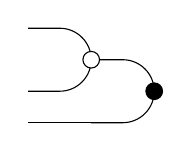
\begin{tikzpicture}[x=0.8cm, y=0.4cm, baseline]
    \draw[rounded corners=0.4cm] (-2,2) -- (-1,2) -- (-1,1);
    \draw[rounded corners=0.4cm] (-2,0) -- (-1,0) -- (-1,1);
    \draw[rounded corners=0.4cm] (-1,1) -- (0,1) -- (0,0);
    \draw[rounded corners=0.4cm] (-1,-1) -- (0,-1) -- (0,0);
    \draw (-1,-1) -- (-2,-1);
    \draw[fill=white] (-1,1) circle (3pt);   
    \draw[fill=black] (0,0) circle (3pt);  
\end{tikzpicture}
\quad=\quad
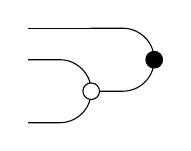
\begin{tikzpicture}[x=0.8cm, y=0.4cm, baseline]
    \draw[rounded corners=0.4cm] (-2,-2) -- (-1,-2) -- (-1,-1);
    \draw[rounded corners=0.4cm] (-2,0) -- (-1,0) -- (-1,-1);
    \draw[rounded corners=0.4cm] (-1,1) -- (0,1) -- (0,0);
    \draw[rounded corners=0.4cm] (-1,-1) -- (0,-1) -- (0,0);
    \draw (-1,1) -- (-2,1);
    \draw[fill=white] (-1,-1) circle (3pt);   
    \draw[fill=black] (0,0) circle (3pt);   
\end{tikzpicture}
\hspace{3em}
\text{(trident map)}
\]

We then show how we are able to express the multiplication through the \emph{trident map} (and the copairing):

\[
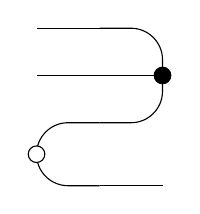
\begin{tikzpicture}[x=0.8cm, y=0.4cm, baseline]
    \draw[rounded corners=0.4cm] (0,0) -- (-1,0) -- (-1,-1);
    \draw[rounded corners=0.4cm] (-1,-1) -- (-1,-2) -- (0,-2);
    \draw (0,-2)--(1,-2);
    \draw[rounded corners=0.4cm] (1,1.5) -- (1,0) -- (0,0);
    \draw[rounded corners=0.4cm] (1,1.5) -- (1,3) -- (0,3);
    \draw (1,1.5) -- (-1,1.5);
    \draw (0,3) -- (-1,3);
    \draw[fill=white] (-1,-1) circle (3pt);   
    \draw[fill=black] (1,1.5) circle (3pt);  
\end{tikzpicture}
\quad=\quad
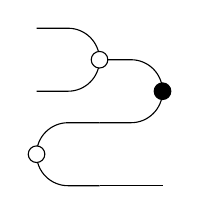
\begin{tikzpicture}[x=0.8cm, y=0.4cm, baseline]
    \draw[rounded corners=0.4cm] (0,0) -- (-1,0) -- (-1,-1);
    \draw[rounded corners=0.4cm] (-1,-1) -- (-1,-2) -- (0,-2);
    \draw (0,-2)--(1,-2);
    \draw[rounded corners=0.4cm] (1,1) -- (1,0) -- (0,0);
    \draw[rounded corners=0.4cm] (1,1) -- (1,2) -- (0,2);
    \draw[rounded corners=0.4cm] (0,2) -- (0,1) -- (-1,1);
    \draw[rounded corners=0.4cm] (0,2) -- (0,3) -- (-1,3);
    \draw[fill=white] (-1,-1) circle (3pt);
    \draw[fill=white] (0,2) circle (3pt);      
    \draw[fill=black] (1,1) circle (3pt); 
\end{tikzpicture}
\quad=\quad
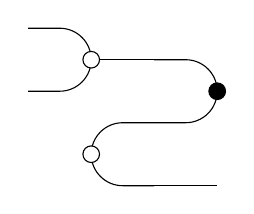
\begin{tikzpicture}[x=0.8cm, y=0.4cm, baseline]
    \draw[rounded corners=0.4cm] (0,0) -- (-1,0) -- (-1,-1);
    \draw[rounded corners=0.4cm] (-1,-1) -- (-1,-2) -- (0,-2);
    \draw (0,-2)--(1,-2);
    \draw[rounded corners=0.4cm] (1,1) -- (1,0) -- (0,0);
    \draw[rounded corners=0.4cm] (1,1) -- (1,2) -- (0,2);
    \draw (0,2) -- (-1,2);
    \draw[rounded corners=0.4cm] (-1,2) -- (-1,1) -- (-2,1);
    \draw[rounded corners=0.4cm] (-1,2) -- (-1,3) -- (-2,3);
    \draw[fill=white] (-1,-1) circle (3pt);
    \draw[fill=white] (-1,2) circle (3pt);      
    \draw[fill=black] (1,1) circle (3pt); 
\end{tikzpicture}
\quad=\quad
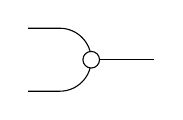
\begin{tikzpicture}[x=0.8cm, y=0.4cm, baseline]
    \draw[rounded corners=0.4cm] (-1,1) -- (0,1) -- (0,0);
    \draw[rounded corners=0.4cm] (-1,-1) -- (0,-1) -- (0,0);
    \draw (0,0) -- (1,0);
    \draw[fill=white] (0,0) circle (3pt); 
\end{tikzpicture}
\]
and
\[
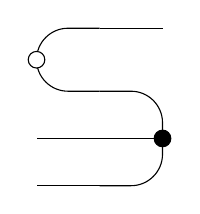
\begin{tikzpicture}[x=0.8cm, y=0.4cm, baseline]
    \draw[rounded corners=0.4cm] (0,0) -- (-1,0) -- (-1,1);
    \draw[rounded corners=0.4cm] (-1,1) -- (-1,2) -- (0,2);
    \draw (0,2)--(1,2);
    \draw[rounded corners=0.4cm] (1,-1.5) -- (1,0) -- (0,0);
    \draw[rounded corners=0.4cm] (1,-1.5) -- (1,-3) -- (0,-3);
    \draw (1,-1.5) -- (-1,-1.5);
    \draw (0,-3) -- (-1,-3);
    \draw[fill=white] (-1,1) circle (3pt);   
    \draw[fill=black] (1,-1.5) circle (3pt);  
\end{tikzpicture}
\quad=\quad
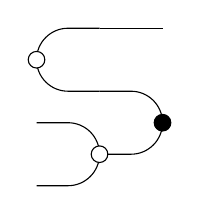
\begin{tikzpicture}[x=0.8cm, y=0.4cm, baseline]
    \draw[rounded corners=0.4cm] (0,0) -- (-1,0) -- (-1,1);
    \draw[rounded corners=0.4cm] (-1,1) -- (-1,2) -- (0,2);
    \draw (0,2)--(1,2);
    \draw[rounded corners=0.4cm] (1,-1) -- (1,0) -- (0,0);
    \draw[rounded corners=0.4cm] (1,-1) -- (1,-2) -- (0,-2);
    \draw[rounded corners=0.4cm] (0,-2) -- (0,-1) -- (-1,-1);
    \draw[rounded corners=0.4cm] (0,-2) -- (0,-3) -- (-1,-3);
    \draw[fill=white] (-1,1) circle (3pt);
    \draw[fill=white] (0,-2) circle (3pt);      
    \draw[fill=black] (1,-1) circle (3pt); 
\end{tikzpicture}
\quad=\quad
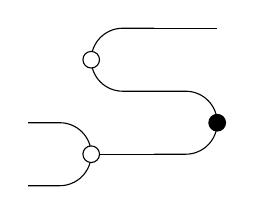
\begin{tikzpicture}[x=0.8cm, y=0.4cm, baseline]
    \draw[rounded corners=0.4cm] (0,0) -- (-1,0) -- (-1,1);
    \draw[rounded corners=0.4cm] (-1,1) -- (-1,2) -- (0,2);
    \draw (0,2)--(1,2);
    \draw[rounded corners=0.4cm] (1,-1) -- (1,0) -- (0,0);
    \draw[rounded corners=0.4cm] (1,-1) -- (1,-2) -- (0,-2);
    \draw (0,-2) -- (-1,-2);
    \draw[rounded corners=0.4cm] (-1,-2) -- (-1,-1) -- (-2,-1);
    \draw[rounded corners=0.4cm] (-1,-2) -- (-1,-3) -- (-2,-3);
    \draw[fill=white] (-1,1) circle (3pt);
    \draw[fill=white] (-1,-2) circle (3pt);      
    \draw[fill=black] (1,-1) circle (3pt); 
\end{tikzpicture}
\quad=\quad
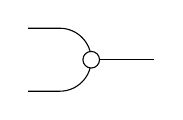
\begin{tikzpicture}[x=0.8cm, y=0.4cm, baseline]
    \draw[rounded corners=0.4cm] (-1,1) -- (0,1) -- (0,0);
    \draw[rounded corners=0.4cm] (-1,-1) -- (0,-1) -- (0,0);
    \draw (0,0) -- (1,0);
    \draw[fill=white] (0,0) circle (3pt); 
\end{tikzpicture}
\]

This gives the following equivalence
\[
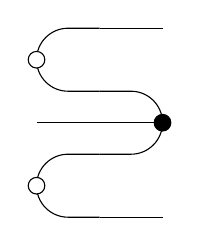
\begin{tikzpicture}[x=0.8cm, y=0.4cm, baseline]
    \draw[rounded corners=0.4cm] (-1,1) -- (0,1) -- (0,0);
    \draw[rounded corners=0.4cm] (-1,-1) -- (0,-1) -- (0,0);
    \draw (0,0) -- (-2,0);
    \draw[rounded corners=0.4cm] (-1,1) -- (-2,1) -- (-2,2);
    \draw[rounded corners=0.4cm] (-1,3) -- (-2,3) -- (-2,2);
    \draw (-1,3) -- (0,3);   
    \draw[rounded corners=0.4cm] (-1,-1) -- (-2,-1) -- (-2,-2);
    \draw[rounded corners=0.4cm] (-2,-2) -- (-2,-3) -- (-1,-3);
    \draw (-1,-3) -- (0,-3);
    \draw[fill=white] (-2,2) circle (3pt);
    \draw[fill=white] (-2,-2) circle (3pt);      
    \draw[fill=black] (0,0) circle (3pt);
\end{tikzpicture}
\quad=\quad
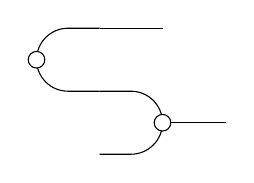
\begin{tikzpicture}[x=0.8cm, y=0.4cm, baseline]
    \draw[rounded corners=0.4cm] (-1,1) -- (-2,1) -- (-2,2);
    \draw[rounded corners=0.4cm] (-1,3) -- (-2,3) -- (-2,2);
    \draw (-1,3) -- (0,3);
    \draw[rounded corners=0.4cm] (-1,1) -- (0,1) -- (0,0);
    \draw[rounded corners=0.4cm] (-1,-1) -- (0,-1) -- (0,0);
    \draw (0,0)--(1,0);
    \draw[fill=white] (0,0) circle (3pt);    
    \draw[fill=white] (-2,2) circle (3pt);    
\end{tikzpicture}
\quad=\quad
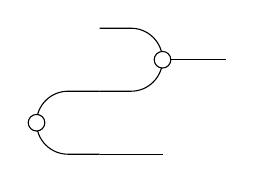
\begin{tikzpicture}[x=0.8cm, y=0.4cm, baseline]
    \draw[rounded corners=0.4cm] (-1,-1) -- (-2,-1) -- (-2,-2);
    \draw[rounded corners=0.4cm] (-2,-2) -- (-2,-3) -- (-1,-3);
    \draw (-1,-3) -- (0,-3);
    \draw[rounded corners=0.4cm] (-1,1) -- (0,1) -- (0,0);
    \draw[rounded corners=0.4cm] (-1,-1) -- (0,-1) -- (0,0);
    \draw (0,0)--(1,0);
    \draw[fill=white] (0,0) circle (3pt);  
    \draw[fill=white] (-2,-2) circle (3pt);      
\end{tikzpicture}
\quad=\colon\quad
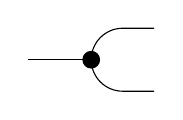
\begin{tikzpicture}[x=0.8cm, y=0.4cm, baseline]
    \draw[rounded corners=0.4cm] (0,0)--(0,1)--(1,1);
    \draw[rounded corners=0.4cm] (0,0)--(0,-1)--(1,-1);
    \draw (0,0) -- (-1,0);
    \draw[fill=black] (0,0) circle (3pt);
\end{tikzpicture}
\]
through which we finally define a \emph{comultiplication} $\delta \colon A \to A \tensor A$ in terms of $\mu$ and $\gamma$. 

The converse also holds: the multiplication can be written in terms of comultiplication and pairing. We omit an explicit proof as it follows the same pattern as the previous one.

\[
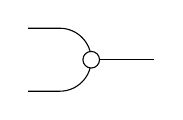
\begin{tikzpicture}[x=0.8cm, y=0.4cm, baseline]
    \draw[rounded corners=0.4cm] (0,0)--(0,1)--(-1,1);
    \draw[rounded corners=0.4cm] (0,0)--(0,-1)--(-1,-1);
    \draw (0,0) -- (1,0);
    \draw[fill=white] (0,0) circle (3pt);
\end{tikzpicture}
\quad=\quad
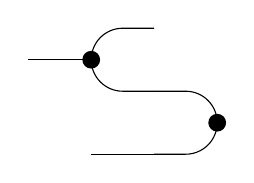
\begin{tikzpicture}[x=0.8cm, y=0.4cm, baseline]
    \draw[rounded corners=0.4cm] (1,-1) -- (2,-1) -- (2,-2);
    \draw[rounded corners=0.4cm] (2,-2) -- (2,-3) -- (1,-3);
    \draw (1,-3) -- (0,-3);
    \draw[rounded corners=0.4cm] (1,1) -- (0,1) -- (0,0);
    \draw[rounded corners=0.4cm] (1,-1) -- (0,-1) -- (0,0);
    \draw (0,0)--(-1,0);
    \draw[fill=black] (0,0) circle (3pt);  
    \draw[fill=black] (2,-2) circle (3pt);      
\end{tikzpicture}
\quad=\quad
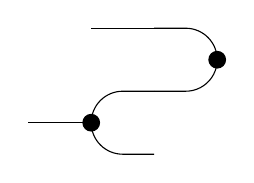
\begin{tikzpicture}[x=0.8cm, y=0.4cm, baseline]
    \draw[rounded corners=0.4cm] (1,1) -- (2,1) -- (2,2);
    \draw[rounded corners=0.4cm] (1,3) -- (2,3) -- (2,2);
    \draw (1,3) -- (0,3);
    \draw[rounded corners=0.4cm] (1,1) -- (0,1) -- (0,0);
    \draw[rounded corners=0.4cm] (1,-1) -- (0,-1) -- (0,0);
    \draw (0,0)--(-1,0);
    \draw[fill=black] (0,0) circle (3pt);    
    \draw[fill=black] (2,2) circle (3pt);    
\end{tikzpicture}
\]


\textbf{(Defining a coalgebra).} To show that this map, together with the Frobenius form $\varepsilon \colon A \to \Bbbk$, defines a coalgebra we need to prove the coassociativity and counit axioms.

For the coassociativity, we start by unwinding the two comultiplications
\[
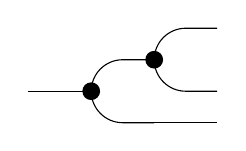
\begin{tikzpicture}[x=0.8cm, y=0.4cm, baseline]
    \draw[rounded corners=0.4cm] (2,2) -- (1,2) -- (1,1);
    \draw[rounded corners=0.4cm] (2,0) -- (1,0) -- (1,1);
    \draw[rounded corners=0.4cm] (1,1) -- (0,1) -- (0,0);
    \draw[rounded corners=0.4cm] (1,-1) -- (0,-1) -- (0,0);
    \draw (0,0) -- (-1,0);
    \draw (1,-1) -- (2,-1);
    \draw[fill=black] (1,1) circle (3pt);   
    \draw[fill=black] (0,0) circle (3pt);  
\end{tikzpicture}
\quad\overset{\text{def}}{=}\quad
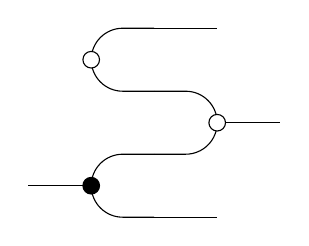
\begin{tikzpicture}[x=0.8cm, y=0.4cm, baseline]
    \draw[rounded corners=0.4cm] (1,1) -- (0,1) -- (0,0);
    \draw[rounded corners=0.4cm] (1,-1) -- (0,-1) -- (0,0);
    \draw (0,0) -- (-1,0);
    \draw (1,-1) -- (2,-1);
    \draw[fill=black] (0,0) circle (3pt); 
    \draw[rounded corners=0.4cm] (2,2) -- (2,1) -- (1,1);
    \draw[rounded corners=0.4cm] (2,2) -- (2,3) -- (1,3);
    \draw (2,2)--(3,2);
    \draw[rounded corners=0.4cm] (0,4) -- (0,3) -- (1,3);   
    \draw[rounded corners=0.4cm] (0,4) -- (0,5) -- (1,5);
    \draw (1,5) -- (2,5);
    \draw[fill=white] (2,2) circle (3pt); 
    \draw[fill=white] (0,4) circle (3pt); 
\end{tikzpicture}
\quad=\quad
\begin{tikzpicture}[x=0.8cm, y=0.4cm, baseline]
    \draw[rounded corners=0.4cm] (2,2) -- (2,1) -- (1,1);
    \draw[rounded corners=0.4cm] (2,2) -- (2,3) -- (1,3);
    \draw (2,2)--(3,2);
    \draw[rounded corners=0.4cm] (0,4) -- (0,3) -- (1,3);   
    \draw[rounded corners=0.4cm] (0,4) -- (0,5) -- (1,5);
    \draw[fill=white] (2,2) circle (3pt); 
    \draw[fill=white] (0,4) circle (3pt); 
    \draw (1,1) -- (0,1);
    \draw[rounded corners=0.4cm] (-1,2) -- (0,2) -- (0,1);
    \draw[rounded corners=0.4cm] (-1,0) -- (0,0) -- (0,1);
    \draw[rounded corners=0.4cm] (-2,-1) -- (-2,0) -- (-1,0);
    \draw[rounded corners=0.4cm] (-2,-1) -- (-2,-2) -- (-1,-2);
    \draw (0,-2) -- (-1,-2);
    \draw[fill=white] (-2,-1) circle (3pt); 
    \draw[fill=white] (0,1) circle (3pt); 
\end{tikzpicture}
\quad=
\]

Then, using the associativity of the multiplication, we get
\[
=\quad
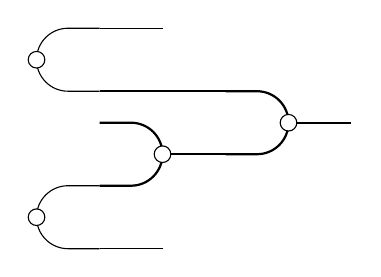
\begin{tikzpicture}[x=0.8cm, y=0.4cm, baseline]
    \draw[rounded corners=0.4cm, thick] (2,2) -- (2,1) -- (1,1);
    \draw[rounded corners=0.4cm, thick] (2,2) -- (2,3) -- (1,3);
    \draw[thick] (2,2)--(3,2);
    \draw[rounded corners=0.4cm] (-2,4) -- (-2,3) -- (-1,3);   
    \draw[rounded corners=0.4cm] (-2,4) -- (-2,5) -- (-1,5);
    \draw (-1,5) -- (0,5);
    \draw[thick] (-1,3) -- (1,3); 
    \draw[fill=white] (2,2) circle (3pt); 
    \draw[fill=white] (-2,4) circle (3pt); 
    \draw[thick] (1,1) -- (0,1);
    \draw[rounded corners=0.4cm, thick] (-1,2) -- (0,2) -- (0,1);
    \draw[rounded corners=0.4cm, thick] (-1,0) -- (0,0) -- (0,1);
    \draw[rounded corners=0.4cm] (-2,-1) -- (-2,0) -- (-1,0);
    \draw[rounded corners=0.4cm] (-2,-1) -- (-2,-2) -- (-1,-2);
    \draw (0,-2) -- (-1,-2);
    \draw[fill=white] (-2,-1) circle (3pt); 
    \draw[fill=white] (0,1) circle (3pt); 
\end{tikzpicture}
\quad=\quad
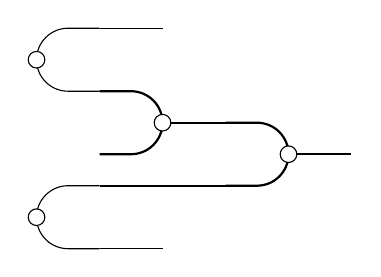
\begin{tikzpicture}[x=0.8cm, y=0.4cm, baseline]
    \draw[rounded corners=0.4cm, thick] (2,1) -- (2,0) -- (1,0);
    \draw[rounded corners=0.4cm, thick] (2,1) -- (2,2) -- (1,2);
    \draw[thick] (2,1)--(3,1);
    \draw[thick] (0,2)--(1,2);
    \draw[rounded corners=0.4cm] (-2,4) -- (-2,3) -- (-1,3);   
    \draw[rounded corners=0.4cm] (-2,4) -- (-2,5) -- (-1,5);
    \draw (-1,5) -- (0,5);
    \draw[fill=white] (2,1) circle (3pt); 
    \draw[fill=white] (-2,4) circle (3pt); 
    \draw[thick] (1,0) -- (-1,0);
    \draw[rounded corners=0.4cm, thick] (-1,3) -- (0,3) -- (0,2);
    \draw[rounded corners=0.4cm, thick] (-1,1) -- (0,1) -- (0,2);
    \draw[rounded corners=0.4cm] (-2,-1) -- (-2,0) -- (-1,0);
    \draw[rounded corners=0.4cm] (-2,-1) -- (-2,-2) -- (-1,-2);
    \draw (0,-2) -- (-1,-2);
    \draw[fill=white] (-2,-1) circle (3pt); 
    \draw[fill=white] (0,2) circle (3pt); 
\end{tikzpicture}
\quad=
\]

in which we can identify the definition of comultiplication hence rewrite it as

\[
=\quad
\begin{tikzpicture}[x=0.8cm, y=0.4cm, baseline]
    \draw[rounded corners=0.4cm] (2,-2) -- (2,-1) -- (1,-1);
    \draw[rounded corners=0.4cm] (2,-2) -- (2,-3) -- (1,-3);
    \draw (2,-2)--(3,-2);
    \draw[rounded corners=0.4cm] (0,-4) -- (0,-3) -- (1,-3);   
    \draw[rounded corners=0.4cm] (0,-4) -- (0,-5) -- (1,-5);
    \draw[fill=white] (2,-2) circle (3pt); 
    \draw[fill=white] (0,-4) circle (3pt); 
    \draw (1,-1) -- (0,-1);
    \draw[rounded corners=0.4cm] (-1,-2) -- (0,-2) -- (0,-1);
    \draw[rounded corners=0.4cm] (-1,0) -- (0,0) -- (0,-1);
    \draw[rounded corners=0.4cm] (-2,1) -- (-2,0) -- (-1,0);
    \draw[rounded corners=0.4cm] (-2,1) -- (-2,2) -- (-1,2);
    \draw (0,2) -- (-1,2);
    \draw[fill=white] (-2,1) circle (3pt); 
    \draw[fill=white] (0,-1) circle (3pt); 
\end{tikzpicture}
\quad=\quad
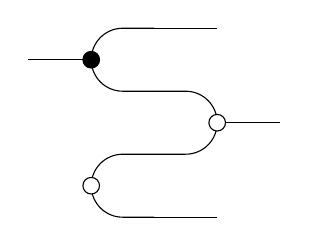
\begin{tikzpicture}[x=0.8cm, y=0.4cm, baseline]
    \draw[rounded corners=0.4cm] (1,1) -- (0,1) -- (0,0);
    \draw[rounded corners=0.4cm] (1,-1) -- (0,-1) -- (0,0);
    \draw (0,0) -- (-1,0);
    \draw (1,1) -- (2,1);
    \draw[fill=black] (0,0) circle (3pt); 
    \draw[rounded corners=0.4cm] (2,-2) -- (2,-1) -- (1,-1);
    \draw[rounded corners=0.4cm] (2,-2) -- (2,-3) -- (1,-3);
    \draw (2,-2)--(3,-2);
    \draw[rounded corners=0.4cm] (0,-4) -- (0,-3) -- (1,-3);   
    \draw[rounded corners=0.4cm] (0,-4) -- (0,-5) -- (1,-5);
    \draw (1,-5) -- (2,-5);
    \draw[fill=white] (2,-2) circle (3pt); 
    \draw[fill=white] (0,-4) circle (3pt); 
\end{tikzpicture}
\quad=\quad
\begin{tikzpicture}[x=0.8cm, y=0.4cm, baseline]
    \draw[rounded corners=0.4cm] (2,0) -- (1,0) -- (1,-1);
    \draw[rounded corners=0.4cm] (2,-2) -- (1,-2) -- (1,-1);
    \draw[rounded corners=0.4cm] (1,1) -- (0,1) -- (0,0);
    \draw[rounded corners=0.4cm] (1,-1) -- (0,-1) -- (0,0);
    \draw (0,0) -- (-1,0);
    \draw (1,1) -- (2,1);
    \draw[fill=black] (1,-1) circle (3pt);   
    \draw[fill=black] (0,0) circle (3pt);  
\end{tikzpicture}
\]

We now prove the counit axioms:

\[
\begin{tikzpicture}[x=0.8cm, y=0.4cm, baseline]
    \draw[rounded corners=0.4cm] (2,-1) -- (0,-1) -- (0,0);
    \draw[rounded corners=0.4cm] (1,1) -- (0,1) -- (0,0);
    \draw (0,0) -- (-1,0);
    \draw[fill=black] (0,0) circle (3pt);
    \draw[fill=black] (1,1) circle (3pt);
\end{tikzpicture}
\quad\overset{unit}{=}\quad
\begin{tikzpicture}[x=0.8cm, y=0.4cm, baseline]
    \draw[rounded corners=0.4cm] (2,-1) -- (0,-1) -- (0,0);
    \draw[rounded corners=0.4cm] (1,1) -- (0,1) -- (0,0);
    \draw (0,0) -- (-1,0);
    \draw[fill=black] (0,0) circle (3pt);
    \draw[rounded corners=0.4cm] (2,2) -- (2,1) -- (1,1);
    \draw[rounded corners=0.4cm] (2,2) -- (2,3) -- (1,3);
    \draw[fill=black] (2,2) circle (3pt);
    \draw[fill=white] (1,3) circle (3pt);
\end{tikzpicture}
\quad=\quad
\begin{tikzpicture}[x=0.8cm, y=0.4cm, baseline]
    \draw[rounded corners=0.4cm] (-1,1) -- (0,1) -- (0,0);
    \draw[rounded corners=0.4cm] (-1,-1) -- (0,-1) -- (0,0);
    \draw (-1,-1) -- (-2,-1);
    \draw (0,0) -- (1,0);
    \draw[fill=white] (0,0) circle (3pt);
    \draw[fill=white] (-1,1) circle (3pt);
\end{tikzpicture}
\quad=\quad
\begin{tikzpicture}[x=0.8cm, y=0.4cm, baseline]
    \draw (0,0) -- (1,0);    
\end{tikzpicture}
\]
\[
\begin{tikzpicture}[x=0.8cm, y=0.4cm, baseline]
    \draw[rounded corners=0.4cm] (2,1) -- (0,1) -- (0,0);
    \draw[rounded corners=0.4cm] (1,-1) -- (0,-1) -- (0,0);
    \draw (0,0) -- (-1,0);
    \draw[fill=black] (0,0) circle (3pt);
    \draw[fill=black] (1,-1) circle (3pt);
\end{tikzpicture}
\quad\overset{unit}{=}\quad
\begin{tikzpicture}[x=0.8cm, y=0.4cm, baseline]
    \draw[rounded corners=0.4cm] (2,1) -- (0,1) -- (0,0);
    \draw[rounded corners=0.4cm] (1,-1) -- (0,-1) -- (0,0);
    \draw (0,0) -- (-1,0);
    \draw[fill=black] (0,0) circle (3pt);
    \draw[rounded corners=0.4cm] (2,-2) -- (2,-1) -- (1,-1);
    \draw[rounded corners=0.4cm] (2,-2) -- (2,-3) -- (1,-3);
    \draw[fill=black] (2,-2) circle (3pt);
    \draw[fill=white] (1,-3) circle (3pt);
\end{tikzpicture}
\quad=\quad
\begin{tikzpicture}[x=0.8cm, y=0.4cm, baseline]
    \draw[rounded corners=0.4cm] (-1,-1) -- (0,-1) -- (0,0);
    \draw[rounded corners=0.4cm] (-1,1) -- (0,1) -- (0,0);
    \draw (-1,1) -- (-2,1);
    \draw (0,0) -- (1,0);
    \draw[fill=white] (0,0) circle (3pt);
    \draw[fill=white] (-1,-1) circle (3pt);
\end{tikzpicture}
\quad=\quad
\begin{tikzpicture}[x=0.8cm, y=0.4cm, baseline]
    \draw (0,0) -- (1,0);    
\end{tikzpicture}
\]

\textbf{(Frobenius relation).}
Lastly, we show the Frobenius relation is satisfied.

\[
\begin{tikzpicture}[x=0.8cm, y=0.4cm, baseline]
    \draw[rounded corners=0.4cm] (-1,-1) -- (0,-1) -- (0,0);
    \draw[rounded corners=0.4cm] (-1,1) -- (0,1) -- (0,0);
    \draw (0,0) -- (1,0);
    \draw[fill=white] (0,0) circle (3pt);
    \draw[fill=black] (1,0) circle (3pt);
    \draw[rounded corners=0.4cm] (1,0) -- (1,1) -- (2,1);
    \draw[rounded corners=0.4cm] (1,0) -- (1,-1) -- (2,-1);
\end{tikzpicture}
\quad=\quad
\begin{tikzpicture}[x=0.8cm, y=0.4cm, baseline]
    \draw[rounded corners=0.4cm] (-1,-1) -- (0,-1) -- (0,0);
    \draw[rounded corners=0.4cm] (-1,1) -- (0,1) -- (0,0);
    \draw[rounded corners=0.4cm] (1,1) -- (1,0) -- (0,0);
    \draw[rounded corners=0.4cm] (1,1) -- (1,2) -- (0,2);
    \draw (1,1)--(2,1);
    \draw[rounded corners=0.4cm] (-.5,3) -- (-.5,2) -- (.5,2);
    \draw[rounded corners=0.4cm] (-.5,3) -- (-.5,4) -- (.5,4);
    \draw[fill=white] (0,0) circle (3pt);
    \draw[fill=white] (1,1) circle (3pt);
    \draw[fill=white] (-.5,3) circle (3pt);
\end{tikzpicture}
\quad\overset{ass.}{=}\quad
\begin{tikzpicture}[x=0.8cm, y=0.4cm, baseline]
    \draw[rounded corners=0.4cm] (1,1) -- (1,0) -- (0,0);
    \draw[rounded corners=0.4cm] (1,1) -- (1,2) -- (0,2);
    \draw[rounded corners=0.4cm] (-.5,3) -- (-.5,2) -- (.5,2);
    \draw[rounded corners=0.4cm] (-.5,3) -- (-.5,4) -- (1.5,4);
    \draw[rounded corners=0.4cm] (2,0) -- (2,1) -- (1,1);
    \draw[rounded corners=0.4cm] (2,0) -- (2,-1) -- (1,-1);
    \draw (2,0)--(3,0);
    \draw[fill=white] (1,1) circle (3pt);
    \draw[fill=white] (-.5,3) circle (3pt);
    \draw[fill=white] (2,0) circle (3pt);
\end{tikzpicture}
\quad=\quad
\begin{tikzpicture}[x=0.8cm, y=0.4cm, baseline]
    \draw[rounded corners=0.4cm] (0,2) -- (0,1) -- (.5,1);
    \draw[rounded corners=0.4cm] (0,2) -- (0,3) -- (1.5,3);
    \draw[rounded corners=0.4cm] (1,0) -- (1,1) -- (.5,1);
    \draw[rounded corners=0.4cm] (1,0) -- (1,-1) -- (-.5,-1);
    \draw (2,0)--(1,0);
    \draw (0,2)--(-1,2);
    \draw[fill=black] (0,2) circle (3pt);
    \draw[fill=white] (1,0) circle (3pt);
\end{tikzpicture}
\]

\[
\begin{tikzpicture}[x=0.8cm, y=0.4cm, baseline]
    \draw[rounded corners=0.4cm] (-1,-1) -- (0,-1) -- (0,0);
    \draw[rounded corners=0.4cm] (-1,1) -- (0,1) -- (0,0);
    \draw (0,0) -- (1,0);
    \draw[fill=white] (0,0) circle (3pt);
    \draw[fill=black] (1,0) circle (3pt);
    \draw[rounded corners=0.4cm] (1,0) -- (1,1) -- (2,1);
    \draw[rounded corners=0.4cm] (1,0) -- (1,-1) -- (2,-1);
\end{tikzpicture}
\quad=\quad
\begin{tikzpicture}[x=0.8cm, y=0.4cm, baseline]
    \draw[rounded corners=0.4cm] (-1,1) -- (0,1) -- (0,0);
    \draw[rounded corners=0.4cm] (-1,-1) -- (0,-1) -- (0,0);
    \draw[rounded corners=0.4cm] (1,-1) -- (1,0) -- (0,0);
    \draw[rounded corners=0.4cm] (1,-1) -- (1,-2) -- (0,-2);
    \draw (1,-1)--(2,-1);
    \draw[rounded corners=0.4cm] (-.5,-3) -- (-.5,-2) -- (.5,-2);
    \draw[rounded corners=0.4cm] (-.5,-3) -- (-.5,-4) -- (.5,-4);
    \draw[fill=white] (0,0) circle (3pt);
    \draw[fill=white] (1,-1) circle (3pt);
    \draw[fill=white] (-.5,-3) circle (3pt);
\end{tikzpicture}
\quad\overset{ass.}{=}\quad
\begin{tikzpicture}[x=0.8cm, y=0.4cm, baseline]
    \draw[rounded corners=0.4cm] (1,-1) -- (1,0) -- (0,0);
    \draw[rounded corners=0.4cm] (1,-1) -- (1,-2) -- (0,-2);
    \draw[rounded corners=0.4cm] (-.5,-3) -- (-.5,-2) -- (.5,-2);
    \draw[rounded corners=0.4cm] (-.5,-3) -- (-.5,-4) -- (.5,-4);
    \draw[rounded corners=0.4cm] (2,0) -- (2,-1) -- (1,-1);
    \draw[rounded corners=0.4cm] (2,0) -- (2,1) -- (1,1);
    \draw (2,0)--(3,0);
    \draw[fill=white] (1,-1) circle (3pt);
    \draw[fill=white] (-.5,-3) circle (3pt);
    \draw[fill=white] (2,0) circle (3pt);
\end{tikzpicture}
\quad=\quad
\begin{tikzpicture}[x=0.8cm, y=0.4cm, baseline]
    \draw[rounded corners=0.4cm] (0,-2) -- (0,-1) -- (.5,-1);
    \draw[rounded corners=0.4cm] (0,-2) -- (0,-3) -- (1.5,-3);
    \draw[rounded corners=0.4cm] (1,0) -- (1,-1) -- (.5,-1);
    \draw[rounded corners=0.4cm] (1,0) -- (1,1) -- (-.5,1);
    \draw (1,0)--(2,0);
    \draw (0,-2)--(-1,-2);
    \draw[fill=black] (0,-2) circle (3pt);
    \draw[fill=white] (1,0) circle (3pt);
\end{tikzpicture}
\]

\textbf{(Uniqueness of the comultiplication).}
To simplify some of the next drawings, we notice that the relation between $\gamma$ (copairing) and $\eta$ (unit) is dual to the relation between the Frobenius pairing and the Frobenius form.
\[
\begin{tikzpicture}[x=0.8cm, y=0.4cm, baseline]
    \draw[rounded corners=0.4cm] (1,1) -- (0,1) -- (0,0);
    \draw[rounded corners=0.4cm] (1,-1) -- (0,-1) -- (0,0);
    \draw (0,0) -- (-1,0);
    \draw[fill=black] (0,0) circle (3pt); 
    \draw[fill=white] (-1,0) circle (3pt); 
\end{tikzpicture}
\quad=\quad
\begin{tikzpicture}[x=0.8cm, y=0.4cm, baseline]
    \draw[rounded corners=0.4cm] (1,1) -- (0,1) -- (0,0);
    \draw[rounded corners=0.4cm] (1,-1) -- (0,-1) -- (0,0);
    \draw[fill=white] (0,0) circle (3pt);   
\end{tikzpicture}
\quad\text{and}\quad
\begin{tikzpicture}[x=0.8cm, y=0.4cm, baseline]
    \draw[rounded corners=0.4cm] (1,1) -- (0,1) -- (0,0);
    \draw[rounded corners=0.4cm] (1,-1) -- (0,-1) -- (0,0);
    \draw (1,-1) -- (2,-1);
    \draw[fill=white] (0,0) circle (3pt);
    \draw[fill=black] (1,1) circle (3pt);
\end{tikzpicture}
\quad=\quad
\begin{tikzpicture}[x=0.8cm, y=0.4cm, baseline]
    \draw (0,0) -- (-1,0); 
    \draw[fill=white] (-1,0) circle (3pt);   
\end{tikzpicture}
\quad=\quad
\begin{tikzpicture}[x=0.8cm, y=0.4cm, baseline]
    \draw[rounded corners=0.4cm] (1,1) -- (0,1) -- (0,0);
    \draw[rounded corners=0.4cm] (1,-1) -- (0,-1) -- (0,0);
    \draw (1,1) -- (2,1);
    \draw[fill=white] (0,0) circle (3pt);
    \draw[fill=black] (1,-1) circle (3pt);
\end{tikzpicture}
\]
(The first follows from the definition of comultiplication and unit axioms. The second from counit axioms.)\todo[inline]{show??}

Suppose there exists another comultiplication $\omega \colon A \to A \tensor A$, with $\varepsilon$ as counit and satisfying the Frobenius relation. We distinguish it from $\delta$ by representing it with a black square.

\[
\begin{tikzpicture}[x=0.8cm, y=0.4cm, baseline]
    \draw[rounded corners=0.4cm] (-1,-1) -- (0,-1) -- (0,0);
    \draw[rounded corners=0.4cm] (-1,1) -- (0,1) -- (0,0);
    \draw (0,0) -- (1,0);
    \draw[fill=white] (0,0) circle (3pt);
    \draw[fill=black] (0.85,-.3) rectangle (1.15, .3);
    \draw[rounded corners=0.4cm] (1,0) -- (1,1) -- (2,1);
    \draw[rounded corners=0.4cm] (1,0) -- (1,-1) -- (2,-1);
\end{tikzpicture}
\quad=\quad
\begin{tikzpicture}[x=0.8cm, y=0.4cm, baseline, yshift=-.25cm]
    \draw[rounded corners=0.4cm] (0,2) -- (0,1) -- (1,1);
    \draw[rounded corners=0.4cm] (0,2) -- (0,3) -- (2,3);
    \draw[rounded corners=0.4cm] (2,0) -- (2,1) -- (1,1);
    \draw[rounded corners=0.4cm] (2,0) -- (2,-1) -- (0,-1);
    \draw (2,0)--(3,0);
    \draw (0,2)--(-1,2);
    \draw[fill=black] (-.15,1.7) rectangle (.15, 2.3);
    \draw[fill=white] (2,0) circle (3pt);
\end{tikzpicture}
\]
By composing this equation on both sides with unit and counit, we get
\[
\begin{tikzpicture}[x=0.8cm, y=0.4cm, baseline]
    \draw[rounded corners=0.4cm] (-1,-1) -- (0,-1) -- (0,0);
    \draw[rounded corners=0.4cm] (-1,1) -- (0,1) -- (0,0);
    \draw (0,0) -- (1,0);
    \draw[fill=white] (0,0) circle (3pt);
    \draw[fill=black] (0.85,-.3) rectangle (1.15, .3);
    \draw[rounded corners=0.4cm] (1,0) -- (1,1) -- (2,1);
    \draw[rounded corners=0.4cm] (1,0) -- (1,-1) -- (2,-1);
    \draw[fill=white] (-1,1) circle (3pt);
    \draw[fill=black] (2,-1) circle (3pt);
\end{tikzpicture}
\quad=\quad
\begin{tikzpicture}[x=0.8cm, y=0.4cm, baseline, yshift=-.25cm]
    \draw[rounded corners=0.4cm] (0,2) -- (0,1) -- (1,1);
    \draw[rounded corners=0.4cm] (0,2) -- (0,3) -- (2,3);
    \draw[rounded corners=0.4cm] (2,0) -- (2,1) -- (1,1);
    \draw[rounded corners=0.4cm] (2,0) -- (2,-1) -- (0,-1);
    \draw (2,0)--(3,0);
    \draw (0,2)--(-1,2);
    \draw[fill=black] (-.15,1.7) rectangle (.15, 2.3);
    \draw[fill=white] (2,0) circle (3pt);
    \draw[fill=white] (-1,2) circle (3pt);
    \draw[fill=black] (3,0) circle (3pt);
\end{tikzpicture}
\quad\Rightarrow\quad
\begin{tikzpicture}[x=0.8cm, y=0.4cm, baseline]
    \draw (0,0) -- (1,0);    
\end{tikzpicture}
\quad=\quad
\begin{tikzpicture}[x=0.8cm, y=0.4cm, baseline, yshift=-.25cm]
    \draw[rounded corners=0.4cm] (0,2) -- (0,1) -- (1,1);
    \draw[rounded corners=0.4cm] (0,2) -- (0,3) -- (2,3);
    \draw[rounded corners=0.4cm] (2,0) -- (2,1) -- (1,1);
    \draw[rounded corners=0.4cm] (2,0) -- (2,-1) -- (0,-1);
    \draw (0,2)--(-1,2);
    \draw[fill=black] (-.15,1.7) rectangle (.15, 2.3);
    \draw[fill=white] (2,0) circle (3pt);
    \draw[fill=white] (-1,2) circle (3pt);
    \draw[fill=black] (2,0) circle (3pt);
\end{tikzpicture}
\]
By uniqueness of the copairing we can say that $\begin{tikzpicture}[x=0.4cm, y=0.2cm, baseline, yshift=0.2cm]
    \draw[rounded corners=0.2cm] (0,0) -- (0,1) -- (1,1);
    \draw[rounded corners=0.2cm] (0,0) -- (0,-1) -- (1,-1);
    \draw (-1,0)--(0,0);
    \draw[fill=black] (-.15,-.3) rectangle (.15, .3);
    \draw[fill=white] (-1,0) circle (2pt);
\end{tikzpicture} 
= 
\begin{tikzpicture}[x=0.4cm, y=0.2cm, baseline, yshift=0.2cm]
    \draw[rounded corners=0.2cm] (0,0) -- (0,1) -- (1,1);
    \draw[rounded corners=0.2cm] (0,0) -- (0,-1) -- (1,-1);
    \draw[fill=white] (0,0) circle (2pt);
\end{tikzpicture}$ and so we have

\[
\begin{tikzpicture}[x=0.8cm, y=0.4cm, baseline]
    \draw[rounded corners=0.4cm] (0,0) -- (0,1) -- (1,1);
    \draw[rounded corners=0.4cm] (0,0) -- (0,-1) -- (1,-1);
    \draw (-1,0)--(0,0);
    \draw[fill=black] (-.15,-.3) rectangle (.15, .3);
\end{tikzpicture} 
\quad=\quad
\begin{tikzpicture}[x=0.8cm, y=0.4cm, baseline]
    \draw[rounded corners=0.4cm] (-1,-1) -- (0,-1) -- (0,0);
    \draw[rounded corners=0.4cm] (-1,1) -- (0,1) -- (0,0);
    \draw (0,0) -- (1,0);
    \draw[fill=white] (0,0) circle (3pt);
    \draw[fill=black] (0.85,-.3) rectangle (1.15, .3);
    \draw[rounded corners=0.4cm] (1,0) -- (1,1) -- (2,1);
    \draw[rounded corners=0.4cm] (1,0) -- (1,-1) -- (2,-1);
    \draw[fill=white] (-1,1) circle (3pt);
\end{tikzpicture}
\quad=\quad
\begin{tikzpicture}[x=0.8cm, y=0.4cm, baseline, yshift=-.25cm]
    \draw[rounded corners=0.4cm] (0,2) -- (0,1) -- (1,1);
    \draw[rounded corners=0.4cm] (0,2) -- (0,3) -- (2,3);
    \draw[rounded corners=0.4cm] (2,0) -- (2,1) -- (1,1);
    \draw[rounded corners=0.4cm] (2,0) -- (2,-1) -- (0,-1);
    \draw (2,0)--(3,0);
    \draw (0,2)--(-1,2);
    \draw[fill=black] (-.15,1.7) rectangle (.15, 2.3);
    \draw[fill=white] (2,0) circle (3pt);
    \draw[fill=white] (-1,2) circle (3pt);
\end{tikzpicture}
\quad=\quad
\begin{tikzpicture}[x=0.8cm, y=0.4cm, baseline, yshift=-.25cm]
    \draw[rounded corners=0.4cm] (0,2) -- (0,1) -- (1,1);
    \draw[rounded corners=0.4cm] (0,2) -- (0,3) -- (2,3);
    \draw[rounded corners=0.4cm] (2,0) -- (2,1) -- (1,1);
    \draw[rounded corners=0.4cm] (2,0) -- (2,-1) -- (0,-1);
    \draw (2,0)--(3,0);
    \draw[fill=white] (2,0) circle (3pt);
    \draw[fill=white] (0,2) circle (3pt);
\end{tikzpicture}
\]

which corresponds to the definition of $\delta$. We have proved the comultiplication is unique.

\subsection{From Frobenius relation to pairing}
We now start with considering a vector space $A$ equipped with 
\[
\begin{tikzpicture}[x=0.8cm, y=0.4cm, baseline]
    \draw (0,0)--(1,0);
    \draw[fill=white] (0,0) circle (3pt);
    \node (t1) at (0.5,-2) {$\eta \colon \Bbbk \to A$};
\end{tikzpicture}
\hspace{3em}
\begin{tikzpicture}[x=0.8cm, y=0.4cm, baseline]
    \draw[rounded corners=0.4cm] (0,0)--(0,1)--(-1,1);
    \draw[rounded corners=0.4cm] (0,0)--(0,-1)--(-1,-1);
    \draw (0,0) -- (1,0);
    \draw[fill=white] (0,0) circle (3pt);
    \node (t1) at (0,-2) {$\mu \colon A \tensor A \to A$};
\end{tikzpicture}
\hspace{3em}
\begin{tikzpicture}[x=0.8cm, y=0.4cm, baseline]
    \draw (0,0)--(1,0);
    \draw[fill=black] (1,0) circle (3pt);
    \node (t1) at (0.5,-2) {$\varepsilon \colon A \to \Bbbk$};
\end{tikzpicture}
\hspace{3em}
\begin{tikzpicture}[x=0.8cm, y=0.4cm, baseline]
    \draw[rounded corners=0.4cm] (0,0) -- (0,1) -- (1,1);
    \draw[rounded corners=0.4cm] (0,0) -- (0,-1) -- (1,-1);
    \draw (-1,0)--(0,0);
    \draw[fill=black] (0,0) circle (3pt);
    \node (t1) at (0,-2) {$\delta \colon A \to A \tensor A$};
\end{tikzpicture} 
\]
such that the following three relations are satisfied.
\[
\begin{tikzpicture}[x=0.8cm, y=0.4cm, baseline,yshift=-0.25cm]
    \draw[rounded corners=0.4cm] (0,2) -- (0,1) -- (.5,1);
    \draw[rounded corners=0.4cm] (0,2) -- (0,3) -- (2,3);
    \draw[rounded corners=0.4cm] (1,0) -- (1,1) -- (.5,1);
    \draw[rounded corners=0.4cm] (1,0) -- (1,-1) -- (-1,-1);
    \draw (2,0)--(1,0);
    \draw (0,2)--(-1,2);
    \draw[fill=black] (0,2) circle (3pt);
    \draw[fill=white] (1,0) circle (3pt);
\end{tikzpicture}
\quad=\quad
\begin{tikzpicture}[x=0.8cm, y=0.4cm, baseline]
    \draw[rounded corners=0.4cm] (-1,-1) -- (0,-1) -- (0,0);
    \draw[rounded corners=0.4cm] (-1,1) -- (0,1) -- (0,0);
    \draw (0,0) -- (1,0);
    \draw[fill=white] (0,0) circle (3pt);
    \draw[fill=black] (1,0) circle (3pt);
    \draw[rounded corners=0.4cm] (1,0) -- (1,1) -- (2,1);
    \draw[rounded corners=0.4cm] (1,0) -- (1,-1) -- (2,-1);
\end{tikzpicture}
\quad=\quad
\begin{tikzpicture}[x=0.8cm, y=0.4cm, baseline,yshift=-0.25cm]
    \draw[rounded corners=0.4cm] (0,2) -- (0,1) -- (-.5,1);
    \draw[rounded corners=0.4cm] (0,2) -- (0,3) -- (-2,3);
    \draw[rounded corners=0.4cm] (-1,0) -- (-1,1) -- (-.5,1);
    \draw[rounded corners=0.4cm] (-1,0) -- (-1,-1) -- (1,-1);
    \draw (-2,0)--(-1,0);
    \draw (0,2)--(1,2);
    \draw[fill=white] (0,2) circle (3pt);
    \draw[fill=black] (-1,0) circle (3pt);
\end{tikzpicture}
\hspace{3em}
\text{(Frobenius relation)}
\]
\[
\begin{tikzpicture}[x=0.8cm, y=0.4cm, baseline]
    \draw[rounded corners=0.4cm] (-1,1) -- (0,1) -- (0,0);
    \draw[rounded corners=0.4cm] (-1,-1) -- (0,-1) -- (0,0);
    \draw (-1,-1) -- (-2,-1);
    \draw (0,0) -- (1,0);
    \draw[fill=white] (0,0) circle (3pt);
    \draw[fill=white] (-1,1) circle (3pt);
\end{tikzpicture}
\quad=\quad
\begin{tikzpicture}[x=0.8cm, y=0.4cm, baseline]
    \draw (0,0) -- (1,0);    
\end{tikzpicture}
\quad=\quad
\begin{tikzpicture}[x=0.8cm, y=0.4cm, baseline]
    \draw[rounded corners=0.4cm] (-1,1) -- (0,1) -- (0,0);
    \draw[rounded corners=0.4cm] (-1,-1) -- (0,-1) -- (0,0);
    \draw (-1,1) -- (-2,1);
    \draw (0,0) -- (1,0);
    \draw[fill=white] (0,0) circle (3pt);
    \draw[fill=white] (-1,-1) circle (3pt);
\end{tikzpicture}
\hspace{5em}
\text{(unit axiom)}
\]
\[
\begin{tikzpicture}[x=0.8cm, y=0.4cm, baseline]
    \draw[rounded corners=0.4cm] (1,1) -- (0,1) -- (0,0);
    \draw[rounded corners=0.4cm] (1,-1) -- (0,-1) -- (0,0);
    \draw (1,-1) -- (2,-1);
    \draw (0,0) -- (-1,0);
    \draw[fill=black] (0,0) circle (3pt);
    \draw[fill=black] (1,1) circle (3pt);
\end{tikzpicture}
\quad=\quad
\begin{tikzpicture}[x=0.8cm, y=0.4cm, baseline]
    \draw (0,0) -- (1,0);    
\end{tikzpicture}
\quad=\quad
\begin{tikzpicture}[x=0.8cm, y=0.4cm, baseline]
    \draw[rounded corners=0.4cm] (1,1) -- (0,1) -- (0,0);
    \draw[rounded corners=0.4cm] (1,-1) -- (0,-1) -- (0,0);
    \draw (1,1) -- (2,1);
    \draw (0,0) -- (-1,0);
    \draw[fill=black] (0,0) circle (3pt);
    \draw[fill=black] (1,-1) circle (3pt);
\end{tikzpicture}
\hspace{4em}
\text{(counit axiom)}
\]

Now, by defining the maps 
\[
\begin{tikzpicture}
\begin{scope}[x=0.8cm, y=0.4cm, baseline]
    \draw[rounded corners=0.4cm] (0,0)--(0,1)--(-1,1);
    \draw[rounded corners=0.4cm] (0,0)--(0,-1)--(-1,-1);
    \draw[fill=black] (0,0) circle (3pt);
    \node (eq) at (1,0) {$\colon=$};
\end{scope}
\begin{scope}[x=0.8cm, y=0.4cm, baseline, xshift=2.5cm]
    \draw[rounded corners=0.4cm] (0,0)--(0,1)--(-1,1);
    \draw[rounded corners=0.4cm] (0,0)--(0,-1)--(-1,-1);
    \draw (0,0) -- (1,0);
    \draw[fill=white] (0,0) circle (3pt);
    \draw[fill=black] (1,0) circle (3pt);
\end{scope}
\begin{scope}[x=0.8cm, y=0.4cm, baseline, xshift=1cm, yshift=-1cm]
    \node (eq) at (0,0) {$\beta \colon= \varepsilon \circ \mu$};
\end{scope}
\end{tikzpicture}
\hspace{5em}
\begin{tikzpicture}
\begin{scope}[x=0.8cm, y=0.4cm, baseline]
    \draw[rounded corners=0.4cm] (0,0)--(0,1)--(1,1);
    \draw[rounded corners=0.4cm] (0,0)--(0,-1)--(1,-1);
    \draw[fill=white] (0,0) circle (3pt);
    \node (eq) at (2,0) {$\colon=$};
\end{scope}
\begin{scope}[x=0.8cm, y=0.4cm, baseline, xshift=2.5cm]
    \draw[rounded corners=0.4cm] (0,0)--(0,1)--(1,1);
    \draw[rounded corners=0.4cm] (0,0)--(0,-1)--(1,-1);
    \draw (0,0) -- (-1,0);
    \draw[fill=black] (0,0) circle (3pt);
    \draw[fill=white] (-1,0) circle (3pt);
\end{scope}
\begin{scope}[x=0.8cm, y=0.4cm, baseline, xshift=2cm, yshift=-1cm]
    \node (eq) at (0,0) {$\gamma \colon= \delta \circ \eta$};
\end{scope}
\end{tikzpicture}
\]
we obtain a Frobenius pairing on the algebra $A$.

\textbf{(Non-degeneracy of the pairing).} Taking the Frobenius relation, we can compose both sides with $\eta$ and $\varepsilon$ as depicted below.
\[
\begin{tikzpicture}[x=0.8cm, y=0.4cm, baseline,yshift=-0.25cm]
    \draw[rounded corners=0.4cm] (0,2) -- (0,1) -- (.5,1);
    \draw[rounded corners=0.4cm] (0,2) -- (0,3) -- (2,3);
    \draw[rounded corners=0.4cm] (1,0) -- (1,1) -- (.5,1);
    \draw[rounded corners=0.4cm] (1,0) -- (1,-1) -- (-1,-1);
    \draw (2,0)--(1,0);
    \draw (0,2)--(-1,2);
    \draw[fill=black] (0,2) circle (3pt);
    \draw[fill=black] (2,0) circle (3pt);
    \draw[fill=white] (-1,2) circle (3pt);
    \draw[fill=white] (1,0) circle (3pt);
\end{tikzpicture}
\quad=\quad
\begin{tikzpicture}[x=0.8cm, y=0.4cm, baseline]
    \draw[rounded corners=0.4cm] (-1,-1) -- (0,-1) -- (0,0);
    \draw[rounded corners=0.4cm] (-1,1) -- (0,1) -- (0,0);
    \draw (0,0) -- (1,0);
    \draw[rounded corners=0.4cm] (1,0) -- (1,1) -- (2,1);
    \draw[rounded corners=0.4cm] (1,0) -- (1,-1) -- (2,-1);
    \draw[fill=white] (0,0) circle (3pt);
    \draw[fill=black] (1,0) circle (3pt);
    \draw[fill=white] (-1,1) circle (3pt);
    \draw[fill=black] (2,-1) circle (3pt);
\end{tikzpicture}
\quad\text{;}\quad
\begin{tikzpicture}[x=0.8cm, y=0.4cm, baseline]
    \draw[rounded corners=0.4cm] (-1,-1) -- (0,-1) -- (0,0);
    \draw[rounded corners=0.4cm] (-1,1) -- (0,1) -- (0,0);
    \draw (0,0) -- (1,0);
    \draw[rounded corners=0.4cm] (1,0) -- (1,1) -- (2,1);
    \draw[rounded corners=0.4cm] (1,0) -- (1,-1) -- (2,-1);
    \draw[fill=white] (0,0) circle (3pt);
    \draw[fill=black] (1,0) circle (3pt);
    \draw[fill=white] (-1,-1) circle (3pt);
    \draw[fill=black] (2,1) circle (3pt);
\end{tikzpicture}
\quad=\quad
\begin{tikzpicture}[x=0.8cm, y=0.4cm, baseline,yshift=-0.25cm]
    \draw[rounded corners=0.4cm] (0,2) -- (0,1) -- (-.5,1);
    \draw[rounded corners=0.4cm] (0,2) -- (0,3) -- (-2,3);
    \draw[rounded corners=0.4cm] (-1,0) -- (-1,1) -- (-.5,1);
    \draw[rounded corners=0.4cm] (-1,0) -- (-1,-1) -- (1,-1);
    \draw (-2,0)--(-1,0);
    \draw (0,2)--(1,2);
    \draw[fill=white] (0,2) circle (3pt);
    \draw[fill=black] (-1,0) circle (3pt);
    \draw[fill=white] (-2,0) circle (3pt);
    \draw[fill=black] (1,2) circle (3pt);
\end{tikzpicture}
\]

By definition of $\beta$ and $\gamma$ and applying the unit and counit axioms we obtain
\[
\begin{tikzpicture}[x=0.8cm, y=0.4cm, baseline]
    \draw[rounded corners=0.4cm] (0,0)--(-1,0)--(-1,1);
    \draw[rounded corners=0.4cm] (0,2)--(-1,2)--(-1,1);
    \draw[rounded corners=0.4cm] (1,-1)--(1,0)--(0,0);
    \draw[rounded corners=0.4cm] (1,-1)--(1,-2)--(0,-2);
    \draw (0,2)--(1,2);
    \draw (0,-2)--(-1,-2);
    \draw[fill=white] (-1,1) circle (3pt);   
    \draw[fill=black] (1,-1) circle (3pt);   
\end{tikzpicture}
\quad=\quad
\begin{tikzpicture}[x=0.8cm, y=0.4cm, baseline]
    \draw (0,0) -- (1,0);    
\end{tikzpicture}
\quad=\quad
\begin{tikzpicture}[x=0.8cm, y=0.4cm, baseline]
    \draw[rounded corners=0.4cm] (0,0)--(1,0)--(1,1);
    \draw[rounded corners=0.4cm] (0,2)--(1,2)--(1,1);
    \draw[rounded corners=0.4cm] (-1,-1)--(-1,0)--(0,0);
    \draw[rounded corners=0.4cm] (-1,-1)--(-1,-2)--(-0,-2);
    \draw (0,2)--(-1,2);
    \draw (0,-2)--(1,-2);
    \draw[fill=white] (-1,-1) circle (3pt);   
    \draw[fill=black] (1,1) circle (3pt);   
\end{tikzpicture}
\]
proving the non-degeneracy of $\beta \colon A \tensor A \to \Bbbk$.

\textbf{(Algebra and coalgebra structure).} By proving the associativity and coassociativity axioms we can state $A$ is equipped with both an algebra and a coalgebra structure. We begin by proving $\mu \colon A \tensor A \to A$ is associative. From the Frobenius relation we have the following equivalences.
\[
\begin{tikzpicture}[x=0.8cm, y=0.4cm, baseline]
    \draw[rounded corners=0.4cm] (0,0)--(0,1)--(-1,1);
    \draw[rounded corners=0.4cm] (0,0)--(0,-1)--(-1,-1);
    \draw (0,0) -- (1,0);
    \draw[fill=white] (0,0) circle (3pt);
\end{tikzpicture}
\quad=\quad
\begin{tikzpicture}[x=0.8cm, y=0.4cm, baseline]
    \draw[rounded corners=0.4cm] (-1,-1) -- (0,-1) -- (0,0);
    \draw[rounded corners=0.4cm] (-1,1) -- (0,1) -- (0,0);
    \draw (0,0) -- (1,0);
    \draw[rounded corners=0.4cm] (1,0) -- (1,1) -- (2,1);
    \draw[rounded corners=0.4cm] (1,0) -- (1,-1) -- (2,-1);
    \draw[fill=white] (0,0) circle (3pt);
    \draw[fill=black] (1,0) circle (3pt);
    \draw[fill=black] (2,-1) circle (3pt);
\end{tikzpicture}
\quad\overset{F}{=}\quad
\begin{tikzpicture}[x=0.8cm, y=0.4cm, baseline,yshift=-0.25cm]
    \draw[rounded corners=0.4cm] (0,2) -- (0,1) -- (.5,1);
    \draw[rounded corners=0.4cm] (0,2) -- (0,3) -- (2,3);
    \draw[rounded corners=0.4cm] (1,0) -- (1,1) -- (.5,1);
    \draw[rounded corners=0.4cm] (1,0) -- (1,-1) -- (-1,-1);
    \draw (2,0)--(1,0);
    \draw (0,2)--(-1,2);
    \draw[fill=black] (0,2) circle (3pt);
    \draw[fill=black] (2,0) circle (3pt);
    \draw[fill=white] (1,0) circle (3pt);
\end{tikzpicture}
\quad=\quad
\begin{tikzpicture}[x=0.8cm, y=0.4cm, baseline,yshift=-0.25cm]
    \draw[rounded corners=0.4cm] (0,2) -- (0,1) -- (.5,1);
    \draw[rounded corners=0.4cm] (0,2) -- (0,3) -- (2,3);
    \draw[rounded corners=0.4cm] (1,0) -- (1,1) -- (.5,1);
    \draw[rounded corners=0.4cm] (1,0) -- (1,-1) -- (-1,-1);
    \draw (0,2)--(-1,2);
    \draw[fill=black] (0,2) circle (3pt);
    \draw[fill=white] (1,0) circle (3pt);
\end{tikzpicture}
\]
Through this equivalent representation of $\mu$, we are now able to prove associativity.
\[
\begin{tikzpicture}[x=0.8cm, y=0.4cm, baseline]
    \draw[rounded corners=0.4cm] (-2,2) -- (-1,2) -- (-1,1);
    \draw[rounded corners=0.4cm] (-2,0) -- (-1,0) -- (-1,1);
    \draw[rounded corners=0.4cm] (-1,1) -- (0,1) -- (0,0);
    \draw[rounded corners=0.4cm] (-1,-1) -- (0,-1) -- (0,0);
    \draw (0,0) -- (1,0);
    \draw (-1,-1) -- (-2,-1);
    \draw[fill=white] (-1,1) circle (3pt);   
    \draw[fill=white] (0,0) circle (3pt);  
\end{tikzpicture}
\quad=\quad
\begin{tikzpicture}[x=0.8cm, y=0.4cm, baseline]
    \draw[rounded corners=0.4cm] (-2,2) -- (-1,2) -- (-1,1);
    \draw[rounded corners=0.4cm] (-2,0) -- (-1,0) -- (-1,1);
    \draw (-1,1)--(0,1);
    \draw[rounded corners=0.4cm] (1,2) -- (0,2) -- (0,1);
    \draw[rounded corners=0.4cm] (0.5,0) -- (0,0) -- (0,1);
    \draw[rounded corners=0.4cm] (0.5,0) -- (1,0) -- (1,-1);
    \draw[rounded corners=0.4cm] (-1,-2) -- (1,-2) -- (1,-1);
    \draw[fill=black] (0,1) circle (3pt);
    \draw[fill=white] (-1,1) circle (3pt);
    \draw[fill=white] (1,-1) circle (3pt);
\end{tikzpicture}
\quad\overset{F}{=}\quad
\begin{tikzpicture}[x=0.8cm, y=0.4cm, baseline]
    \draw (-1.5,1)--(-.5,1);
    \draw[rounded corners=0.4cm] (0,2) -- (-.5,2) -- (-.5,1);
    \draw[rounded corners=0.4cm] (.5,0) -- (-.5,0) -- (-.5,1);
    \draw[rounded corners=0.4cm] (0,2) -- (1,2) -- (1,3);
    \draw[rounded corners=0.4cm] (-1,4) -- (1,4) -- (1,3);
    \draw[rounded corners=0.4cm] (0.5,0) -- (1,0) -- (1,-1);
    \draw[rounded corners=0.4cm] (-1,-2) -- (1,-2) -- (1,-1);
    \draw (1,3)--(2,3);
    \draw[fill=black] (-.5,1) circle (3pt);
    \draw[fill=white] (1,-1) circle (3pt);
    \draw[fill=white] (1,3) circle (3pt);
\end{tikzpicture}
\quad=\quad
\begin{tikzpicture}[x=0.8cm, y=0.4cm, baseline]
    \draw[rounded corners=0.4cm] (-2,-2) -- (-1,-2) -- (-1,-1);
    \draw[rounded corners=0.4cm] (-2,0) -- (-1,0) -- (-1,-1);
    \draw[rounded corners=0.4cm] (-1,1) -- (0,1) -- (0,0);
    \draw[rounded corners=0.4cm] (-1,-1) -- (0,-1) -- (0,0);
    \draw (0,0) -- (1,0);
    \draw (-1,1) -- (-2,1);
    \draw[fill=white] (-1,-1) circle (3pt);   
    \draw[fill=white] (0,0) circle (3pt);   
\end{tikzpicture}
\]
Similarly (by noticing $\begin{tikzpicture}[x=0.4cm, y=0.2cm, baseline, yshift=0.1cm]
    \draw[rounded corners=0.2cm] (0,0) -- (0,1) -- (1,1);
    \draw[rounded corners=0.2cm] (0,0) -- (0,-1) -- (1,-1);
    \draw (-1,0)--(0,0);
    \draw[fill=black] (0,0) circle (2pt);
\end{tikzpicture} 
= 
\begin{tikzpicture}[x=0.4cm, y=0.2cm, baseline, yshift=0.5cm]
    \draw[rounded corners=0.2cm] (0,0) -- (0,-1) -- (-.5,-1);
    \draw[rounded corners=0.2cm] (0,0) -- (0,1) -- (-1,1);
    \draw[rounded corners=0.2cm] (-1,-2) -- (-1,-1) -- (-.5,-1);
    \draw[rounded corners=0.2cm] (-1,-2) -- (-1,-3) -- (1,-3);   
    \draw (0,0)--(1,0); 
    \draw[fill=white] (0,0) circle (2pt);
    \draw[fill=black] (-1,-2) circle (2pt);
\end{tikzpicture}$ ) we are able to prove coassociativity for $\delta$.

\textbf{(Associativity of the pairing).} 
The associativity of $\mu$ is key for proving $\beta$ is associative too.
\[
\begin{tikzpicture}[x=0.8cm, y=0.4cm, baseline]
    \draw[rounded corners=0.4cm] (-2,-2) -- (-1,-2) -- (-1,-1);
    \draw[rounded corners=0.4cm] (-2,0) -- (-1,0) -- (-1,-1);
    \draw[rounded corners=0.4cm] (-1,1) -- (0,1) -- (0,0);
    \draw[rounded corners=0.4cm] (-1,-1) -- (0,-1) -- (0,0);
    \draw (-1,1) -- (-2,1);
    \draw[fill=white] (-1,-1) circle (3pt);   
    \draw[fill=black] (0,0) circle (3pt);   
\end{tikzpicture}
\quad=\quad
\begin{tikzpicture}[x=0.8cm, y=0.4cm, baseline]
    \draw[rounded corners=0.4cm] (-2,-2) -- (-1,-2) -- (-1,-1);
    \draw[rounded corners=0.4cm] (-2,0) -- (-1,0) -- (-1,-1);
    \draw[rounded corners=0.4cm] (-1,1) -- (0,1) -- (0,0);
    \draw[rounded corners=0.4cm] (-1,-1) -- (0,-1) -- (0,0);
    \draw (0,0)--(1,0);
    \draw (-1,1) -- (-2,1);
    \draw[fill=white] (-1,-1) circle (3pt);   
    \draw[fill=white] (0,0) circle (3pt);   
    \draw[fill=black] (1,0) circle (3pt);
\end{tikzpicture}
\quad=\quad
\begin{tikzpicture}[x=0.8cm, y=0.4cm, baseline]
    \draw[rounded corners=0.4cm] (-2,2) -- (-1,2) -- (-1,1);
    \draw[rounded corners=0.4cm] (-2,0) -- (-1,0) -- (-1,1);
    \draw[rounded corners=0.4cm] (-1,1) -- (0,1) -- (0,0);
    \draw[rounded corners=0.4cm] (-1,-1) -- (0,-1) -- (0,0);
    \draw (0,0)--(1,0);
    \draw (-1,-1) -- (-2,-1);
    \draw[fill=white] (-1,1) circle (3pt);   
    \draw[fill=white] (0,0) circle (3pt);   
    \draw[fill=black] (1,0) circle (3pt);
\end{tikzpicture}
\quad=\quad
\begin{tikzpicture}[x=0.8cm, y=0.4cm, baseline]
    \draw[rounded corners=0.4cm] (-2,2) -- (-1,2) -- (-1,1);
    \draw[rounded corners=0.4cm] (-2,0) -- (-1,0) -- (-1,1);
    \draw[rounded corners=0.4cm] (-1,1) -- (0,1) -- (0,0);
    \draw[rounded corners=0.4cm] (-1,-1) -- (0,-1) -- (0,0);
    \draw (-1,-1) -- (-2,-1);
    \draw[fill=white] (-1,1) circle (3pt);   
    \draw[fill=black] (0,0) circle (3pt);
\end{tikzpicture}
\]

Through such wires, we are now able to see the difference between commutative and symmetric Frobenius algebras. A commutative Frobenius algebra will satisfy commutativity and cocommutativity:
\[
\begin{tikzpicture}[x=0.8cm, y=0.4cm, baseline]
    \draw[rounded corners=0.4cm] (-1,1) -- (0,1) -- (0,0);
    \draw[rounded corners=0.4cm] (-1,-1) -- (0,-1) -- (0,0);
    \draw (0,0) -- (1,0);
    \draw (-2,-1) -- (-1,1);
    \draw (-2,1) -- (-1,-1);
    \draw[fill=white] (0,0) circle (3pt);
\end{tikzpicture}
\quad=\quad
\begin{tikzpicture}[x=0.8cm, y=0.4cm, baseline]
    \draw[rounded corners=0.4cm] (-1,1) -- (0,1) -- (0,0);
    \draw[rounded corners=0.4cm] (-1,-1) -- (0,-1) -- (0,0);
    \draw (0,0) -- (1,0);
    \draw[fill=white] (0,0) circle (3pt);
\end{tikzpicture}
\hspace{3em}
\begin{tikzpicture}[x=0.8cm, y=0.4cm, baseline]
    \draw[rounded corners=0.4cm] (0,0) -- (0,1) -- (1,1);
    \draw[rounded corners=0.4cm] (0,0) -- (0,-1) -- (1,-1);
    \draw (-1,0)--(0,0);
    \draw (1,1)--(2,-1);
    \draw (1,-1)--(2,1);
    \draw[fill=black] (0,0) circle (3pt);
\end{tikzpicture} 
\quad=\quad
\begin{tikzpicture}[x=0.8cm, y=0.4cm, baseline]
    \draw[rounded corners=0.4cm] (0,0) -- (0,1) -- (1,1);
    \draw[rounded corners=0.4cm] (0,0) -- (0,-1) -- (1,-1);
    \draw (-1,0)--(0,0);
    \draw[fill=black] (0,0) circle (3pt);
\end{tikzpicture} 
\]
On the other hand, a symmetric Frobenius algebra


\section{A category of Frobenius algebras}

Having established various characterizations of Frobenius algebras in Section $\ref{sec:char-Frobenius}$, we now focus on the morphisms between them. To do so, we will refer to the third (see \ref{dfn:Frobenius-algebra-all}) characterization of a Frobenius algebra.

\begin{tcbdfn}[Frobenius algebra homomorphisms]
    Let $(A, \eta, \mu, \varepsilon, \delta)$ and $(A', \eta', \mu', \varepsilon', \delta')$ be two Frobenius algebra. A \emph{Frobenius algebra homomorphism} $\varphi \colon A \to A'$ is a $\Bbbk$-linear map which is both a $\Bbbk$-algebra homomorphism and a $\Bbbk$-coalgebra homomorphism.
\end{tcbdfn}

In particular, a Frobenius algebra homomorphism preserves the Frobenius form (i.e. $\varepsilon' = \varphi(\varepsilon)$). Together with such morphisms, Frobenius algebra then forma a category, which we name $\mathbf{FAlg}_\Bbbk$.

We now investigate the structure of this category.

\begin{tcblemma}
A Frobenius algebra homomorphism is always invertible in $\mathbf{FAlg}_\Bbbk$. 
\end{tcblemma}

\begin{tcblemma}
The tensor product of two Frobenius algebra is again a Frobenius algebra, giving $\mathbf{FAlg}_\Bbbk$ a monoidal structure.
\end{tcblemma}

\todo[inline]{to prove}
\todo[inline]{to add: a category of commutative Frobenius algebras (tensor of commutative is commutative)}